\documentclass[a4]{article}
\pagestyle{myheadings}

%%%%%%%%%%%%%%%%%%%
% Packages/Macros %
%%%%%%%%%%%%%%%%%%%
\usepackage{mathrsfs}


\usepackage{fancyhdr}
\pagestyle{fancy}
\lhead{}
\chead{}
\rhead{}
\lfoot{}
\cfoot{} 
\rfoot{\normalsize\thepage}
\renewcommand{\headrulewidth}{0pt}
\renewcommand{\footrulewidth}{0pt}
\newcommand{\RomanNumeralCaps}[1]
    {\MakeUppercase{\romannumeral #1}}

\usepackage{amssymb,latexsym}  % Standard packages
\usepackage[utf8]{inputenc}
\usepackage[russian]{babel}
\usepackage{MnSymbol}
\usepackage{mathrsfs}
\usepackage{amsmath,amsthm}
\usepackage{indentfirst}
\usepackage{graphicx}%,vmargin}
\usepackage{graphicx}
\graphicspath{{pictures/}} 
\usepackage{verbatim}
\usepackage{color}
\usepackage[nottoc,numbib]{tocbibind}
\usepackage{float}

\usepackage{listings}
\definecolor{codegreen}{rgb}{0,0.6,0}
\definecolor{codegray}{rgb}{0.5,0.5,0.5}
\definecolor{codepurple}{rgb}{0.58,0,0.82}
\definecolor{backcolour}{rgb}{0.95,0.95,0.92}
 
\lstdefinestyle{mystyle}{
    backgroundcolor=\color{backcolour},   
    commentstyle=\color{codegreen},
    keywordstyle=\color{magenta},
    numberstyle=\tiny\color{codegray},
    stringstyle=\color{codepurple},
    basicstyle=\footnotesize,
    breakatwhitespace=false,         
    breaklines=true,                 
    captionpos=b,                    
    keepspaces=true,                 
    numbers=left,                    
    numbersep=5pt,                  
    showspaces=false,                
    showstringspaces=false,
    showtabs=false,                  
    tabsize=2
}
 
\lstset{style=mystyle}

\usepackage{url}
\urldef\myurl\url{foo%.com}





\DeclareGraphicsExtensions{.pdf,.png,.jpg}% -- настройка картинок

\usepackage{epigraph} %%% to make inspirational quotes.
\usepackage[all]{xy} %for XyPic'a
\usepackage{color} 
\usepackage{amscd} %для коммутативных диграмм
%\usepackage[colorlinks,urlcolor=red]{hyperref}

%\renewcommand{\baselinestretch}{1.5}
%\sloppy
%\usepackage{listings}
%\lstset{numbers=left}
%\setmarginsrb{2cm}{1.5cm}{1cm}{1.5cm}{0pt}{0mm}{0pt}{13mm}


\newtheorem{Lemma}{Лемма}[section]
\newtheorem{Proposition}{Предложение}[section]
\newtheorem{Theorem}{Теорема}[section]
\newtheorem{Corollary}{Следствие}[section]
\newtheorem{Remark}{Замечание}[section]
\newtheorem{Definition}{Определение}[section]
\newtheorem{Designations}{Обозначение}[section]




%%%%%%%%%%%%%%%%%%%%%%% 
%Подготовка оглавления% 
%%%%%%%%%%%%%%%%%%%%%%% 
\usepackage[titles]{tocloft}
\renewcommand{\cftdotsep}{2} %частота точек
\renewcommand\cftsecleader{\cftdotfill{\cftdotsep}}
\renewcommand{\cfttoctitlefont}{\hspace{0.38\textwidth} \LARGE\bfseries} 
\renewcommand{\cftsecaftersnum}{.}
\renewcommand{\cftsubsecaftersnum}{.}
\renewcommand{\cftbeforetoctitleskip}{-1em} 
\renewcommand{\cftaftertoctitle}{\mbox{}\hfill \\ \mbox{}\hfill{\footnotesize Стр.}\vspace{-0.5em}} 
%\renewcommand{\cftchapfont}{\normalsize\bfseries \MakeUppercase{\chaptername} } 
%\renewcommand{\cftsecfont}{\hspace{1pt}} 
\renewcommand{\cftsubsecfont}{\hspace{1pt}} 
%\renewcommand{\cftbeforechapskip}{1em} 
\renewcommand{\cftparskip}{3mm} %определяет величину отступа в оглавлении
\setcounter{tocdepth}{5} 
\renewcommand{\listoffigures}{\begingroup %добавляем номер в список иллюстраций
\tocsection
\tocfile{\listfigurename}{lof}
\endgroup}
\renewcommand{\listoftables}{\begingroup %добавляем номер в список иллюстраций
\tocsection
\tocfile{\listtablename}{lot}
\endgroup}


   
   
%\renewcommand{\thelikesection}{(\roman{likesection})}
%%%%%%%%%%%
% Margins %
%%%%%%%%%%%
\addtolength{\textwidth}{0.7in}
\textheight=630pt
\addtolength{\evensidemargin}{-0.4in}
\addtolength{\oddsidemargin}{-0.4in}
\addtolength{\topmargin}{-0.4in}

%%%%%%%%%%%%%%%%%%%%%%%%%%%%%%%%%%%
%%%%%%Переопределение chapter%%%%%% 
%%%%%%%%%%%%%%%%%%%%%%%%%%%%%%%%%%%
\newcommand{\empline}{\mbox{}\newline} 
\newcommand{\likechapterheading}[1]{ 
\begin{center} 
\textbf{\MakeUppercase{#1}} 
\end{center} 
\empline} 

%%%%%%%Запиливание переопределённого chapter в оглавление%%%%%% 
\makeatletter 
\renewcommand{\@dotsep}{2} 
\newcommand{\l@likechapter}[2]{{\bfseries\@dottedtocline{0}{0pt}{0pt}{#1}{#2}}} 
\makeatother 
\newcommand{\likechapter}[1]{ 
\likechapterheading{#1} 
\addcontentsline{toc}{likechapter}{\MakeUppercase{#1}}} 




\usepackage{xcolor}
\usepackage{hyperref}
\definecolor{linkcolor}{HTML}{000000} % цвет ссылок
\definecolor{urlcolor}{HTML}{3643FF} % цвет гиперссылок
 
\hypersetup{pdfstartview=FitH,  linkcolor=linkcolor,urlcolor=urlcolor, colorlinks=true}

%%%%%%%%%%%%
% Document %
%%%%%%%%%%%%

%%%%%%%%%%%%%%%%%%%%%%%%%%%%%
%%%%%%главы -- section*%%%%%%
%%%%section -- subsection%%%%
%subsection -- subsubsection%
%%%%%%%%%%%%%%%%%%%%%%%%%%%%%
\def \newstr {\medskip \par \noindent} 



\begin{document}
\def\contentsname{\LARGE{Содержание}}
\thispagestyle{empty}
\begin{center} 
\vspace{2cm} 
{\Large \sc Санкт-Петербургский Политехнический}\\
\vspace{2mm}
{\Large \sc Университет} им. {\Large\sc Петра Великого}\\
\vspace{1cm}
{\large \sc Институт прикладной математики и механики\\ 
\vspace{0.5mm}
\textsc{}}\\ 
\vspace{0.5mm}
{\large\sc Кафедра прикладной математики}\\
\vspace{15mm}
%\rule[0.5ex]{\linewidth}{2pt}\vspace*{-\baselineskip}\vspace*{3.2pt} 
%\rule[0.5ex]{\linewidth}{1pt}\\[\baselineskip] 
{\huge \sc Отчёт по лабораторным работм №$1-4$\\
	Исследование распределений
	\vspace{6mm}
	
}
\vspace*{2mm}
%\rule[0.7ex]{\linewidth}{1pt}\vspace*{-\baselineskip}\vspace{3.2pt} 
%\rule[0.5ex]{\linewidth}{2pt}\\ 
\vspace{6cm} 
Студент группы $3630102/70301$ \hfill Камянский Д.В.\\
\vspace{1cm}
Преподаватель \hfill Баженов А. Н.\\
\vspace{20mm} 


\vfill {\large\textsc{Санкт-Петербург}}\\ 
2020 г.
\end{center}

%%%%%%%%%%%%%%%%%%%%%%%%%%%%%%%%%%%%%%%%%%%%%%%%%%%%%%%%%%%%%%%%%%%%%%%%%%%%%%%%%%%%%%%%%%%%%%
%\ \\[4cm]

%\rm
%%%%%%%%%%%%%%%%%%%%%%%%%%%%%%%%%%%%%%%%%%%%%%%%%%%%%%%%%%%%%%%%%%%%%%%%%%%%%%%%%%%%%%%%%%%%%%
\newpage
\pagestyle{plain}

%\begin{center}
%\begin{abstract} 

%\end{abstract}

%\end{center}

\newpage
\tableofcontents{}
\newpage
\listoffigures{}
\listoftables{}
\newpage

\section{Постановка задачи}
Для 5 распределений:
\begin{enumerate}
\item \begin{equation}\label{eqn:normal}
N(x,0,1) = \frac{1}{\sqrt{2\pi}}e^{-\frac{x^2}{2}}
\end{equation} 

\item \begin{equation}\label{eqn:cauchy}
C(x,0,1) = \frac{1}{\pi(1+x^2)}
\end{equation}

\item \begin{equation}\label{eqn:laplace}
L\left( x,0,\frac{1}{\sqrt{2}}\right) = \frac{1}{\sqrt{2}}e^{-\sqrt{2}\vert x\vert}
\end{equation}

\item \begin{equation}\label{eqn:poisson}
P(5,k) = \frac{5^k}{k!}e^{-5}
\end{equation}  

\item \begin{equation}\label{eqn:uniform}
M(x,-\sqrt{3}, \sqrt{3}) = 
\begin{cases}
\frac{1}{2\sqrt{3}} &\vert x\vert \leqslant \sqrt{3}\\
0 &\vert x\vert > \sqrt{3}
\end{cases}
\end{equation}
\end{enumerate}

необходимо было выполнить:
\begin{enumerate}
    \item Сгенерировать выборки размером $ 10,50,1000 $.Построить на одном рисунке гистограмму и график плотности распределения.
    \item  Сгенерировать выборки размером $ 10,100,1000 $. Для каждой выборки вычислить следующие статистические характеристики положения данных: $ \bar{x}, med x, Z_{R},Z_{Q},Z_{tr} $. Повторить такие
    вычисления $1000$ раз для каждой выборки и найти среднее характеристик положения и их квадратов.
    \item Сгенерировать выборки размером $ 20 $ и $1000 $.Для каждого распределения определить долю выбросов экспериментально (сгенерировав выборку, соответствующую распределению $1000$
    раз, и вычислив среднюю долю выбросов) и сравнить с результатами,
    полученными теоретически.
    \item Сгенерировать выборки размером $ 20,60,100 $.	Построить на них эмпирические функции распределения и ядерные оценки плотности распределения на отрезке [−4; 4] для непрерывных
    распределений и на отрезке [6; 14] для распределения Пуассона.
\end{enumerate}



\section{Теория}
\subsection{Плотности распределения вероятностей}

Плотностью распределения вероятностей непрерывной случайной величины называется первая производная от функции распределения. Смысл плотности распределения в том, что она показывает, как часто появляется случайная величина в некоторой окрестности точки при повторении опытов.

\subsection{Характеристики положения}
Характеристики положения дают информацию о расположении значений выборки на числовой прямой и характеризуют этот признак с точки зрения некоторого среднего значения.

\begin{enumerate}
\item Выборочное среднее :
\begin{equation}\label{eqn:average}
\overline{x} = \frac{1}{n}\sum_{i=1}^n x_i \hfill  
\end{equation}
\item Выборочная медиана :
\begin{equation}
med\; x = \begin{cases}
x_{k+1}, & n = 2k+1\\
\frac{1}{2}\left(x_k+x_{k+1}\right), & n = 2k
\end{cases} \hfill  \label{eqn:med}
\end{equation}
\item Полусумма экстремальных значений :
\begin{equation}
Z_R = \frac{1}{2}\left(x_1+x_n\right) \hfill  \label{eqn:mean_extr}
\end{equation}
\item Полусумма квартилей :
\begin{equation}
Z_Q = \frac{1}{2}\left(Z_{\frac{1}{4}}+Z_{\frac{3}{4}}\right) \hfill  \label{eqn:quartiles}
\end{equation}
\item Усечённое среднее :
\begin{equation}
Z_{tr} = \frac{1}{n - 2r}\sum_{i=r+1}^{n-r} x_i \hfill  \label{eqn:cut_mean}
\end{equation}
\end{enumerate}


\subsection{Боксплот Тьюки}

Боксплот Тьюки - график, использующийся в описательной статистике, изображающий одномерное распределение вероятностей.

Границами ящика служат первый и третий квартили, линия в середине
ящика — медиана. Концы усов — края статистически значимой выборки
(без выбросов). Длину «усов» определяют разность первого квартиля и полутора межквартильных расстояний и сумма третьего квартиля и полутора межквартильных расстояний. 

Выбросом в статистике называют результат измерения, выделяющийся из общей выборки.

Правая и левая границы:  $X_{1} = Q_{1} - 1.5(Q_{3} - Q_{1}),\;X_{2} = Q_{3} + 1.5(Q_{3} - Q_{1})$

Теоретическая вероятность выбросов:\\
Для непрерывных распределений:
$P^{t}_{e} = F(X_{1}^{t}) + (1 - F(X_{2}^{t}))$\\
Для дискретных распределений:
$P^{t}_{e} = (F(X_{1}^{t}) - P(x=X_{1}^{t})) + (1 - F(X_{2}^{t}))$

\subsection{Эмпирические функции и ядерные оценки}

Статистическим рядом называется последовательность различных элементов выборки $z_{1}, z_{2}, ... , z_{k}$, расположенных в возрастающем порядке с указанием частот $n_{1}, n_{2}, ... , n_{k}$, с которыми эти элементы содержатся в выборке.

Эмпирическая функция распределения:
\begin{equation}
F^{*}(x) = \dfrac{1}{n}\sum\limits_{z_{i}<x}n_{i}
\end{equation}
Ядерная оценка плотности:
\begin{equation}
f_h(x) = \frac{1}{nh}\sum\limits_{i=1}^nK\left(\frac{x-x_i}{h}\right)\label{eqn:art}
\end{equation}
где $K$ является ядром, а $h>0$ является сглаживающим параметром, и называется шириной полосы.

В данной работе в качестве ядра была выбрана плотность вероятности стандартного нормального распределения:
\begin{equation}
K(x) = \frac{1}{\sqrt{2\pi}}e^{-\frac{x^2}{2}}
\end{equation}

Параметр сглаживания будем выбирать по правилу Сильвермана
\begin{equation}
h_{n} = 1.06*\sigma*n^{-1/5}
\end{equation}
где $ \sigma $ - выборочное стандартное отклонение.

\section{Реализация}
Лабораторная работа была выполнена на языке $Python\;3.8.2$.
Для генерации выборки был использован модуль $stats$ библиотеки $scipy$ для генерации выборок различных распределений и библиотека $matplotlib$ для построения графиков.

\newpage
\section{Результаты}

\subsection{Плотности распределения вероятностей}

\begin{figure}[H]
    \centering
    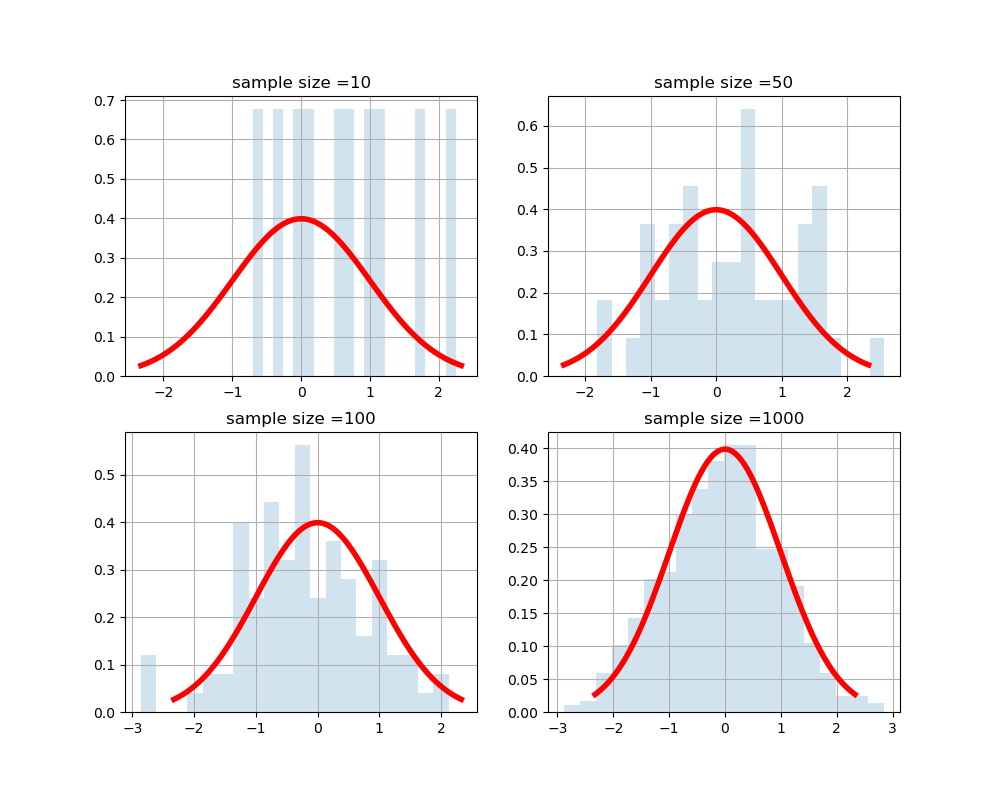
\includegraphics[width=\textwidth]{Lab1_normal.png} 
    \caption{Нормальное распределение \eqref{eqn:normal}}
    \label{fig:dis_norm_gis}
\end{figure}

\begin{figure}[H]
    \centering
    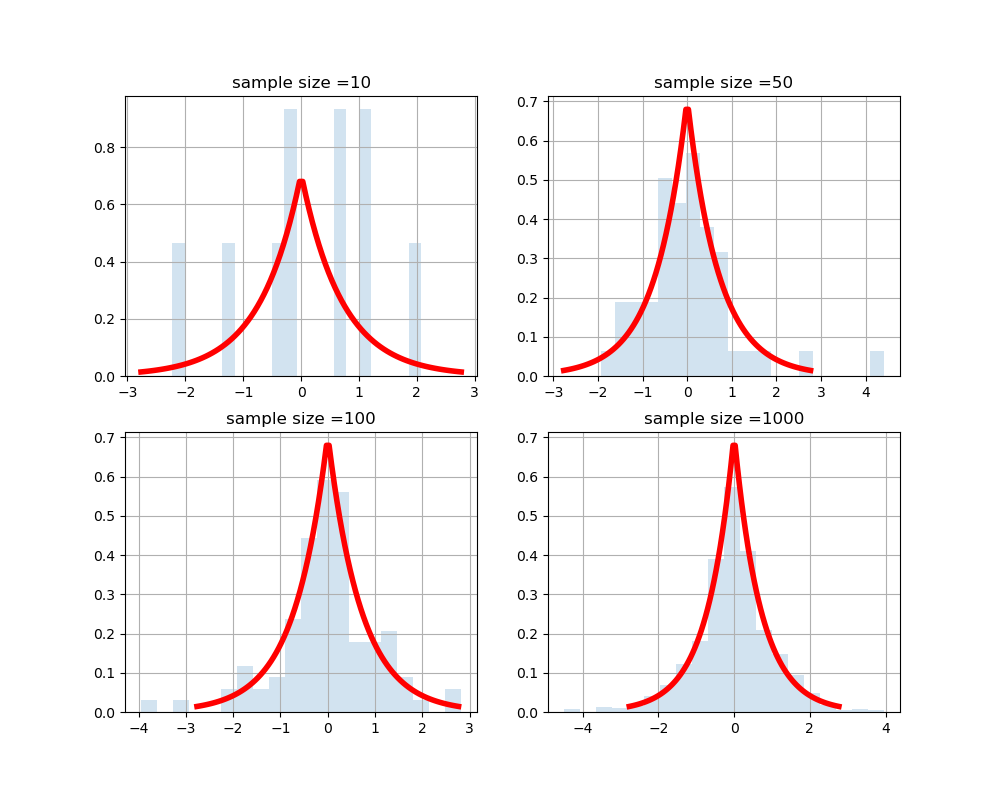
\includegraphics[width=\textwidth]{Lab1_laplace.png}
    \caption{Распределение Лапласа \eqref{eqn:laplace}}
    \label{fig:dis_lapl_gis}
\end{figure}

\begin{figure}[H]
    \centering
    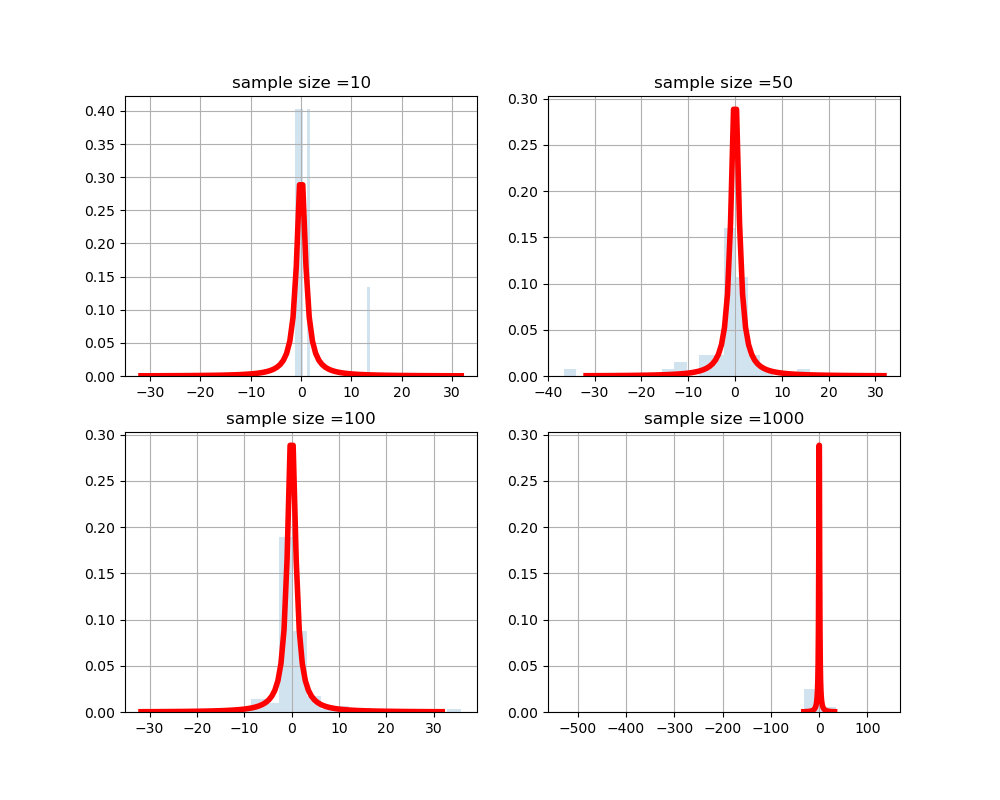
\includegraphics[width=\textwidth]{Lab1_cauchy.png}
    \caption{Распределение Коши \eqref{eqn:cauchy}}
    \label{fig:dis_cauc_gis}
\end{figure}

\begin{figure}[H]
    \centering
    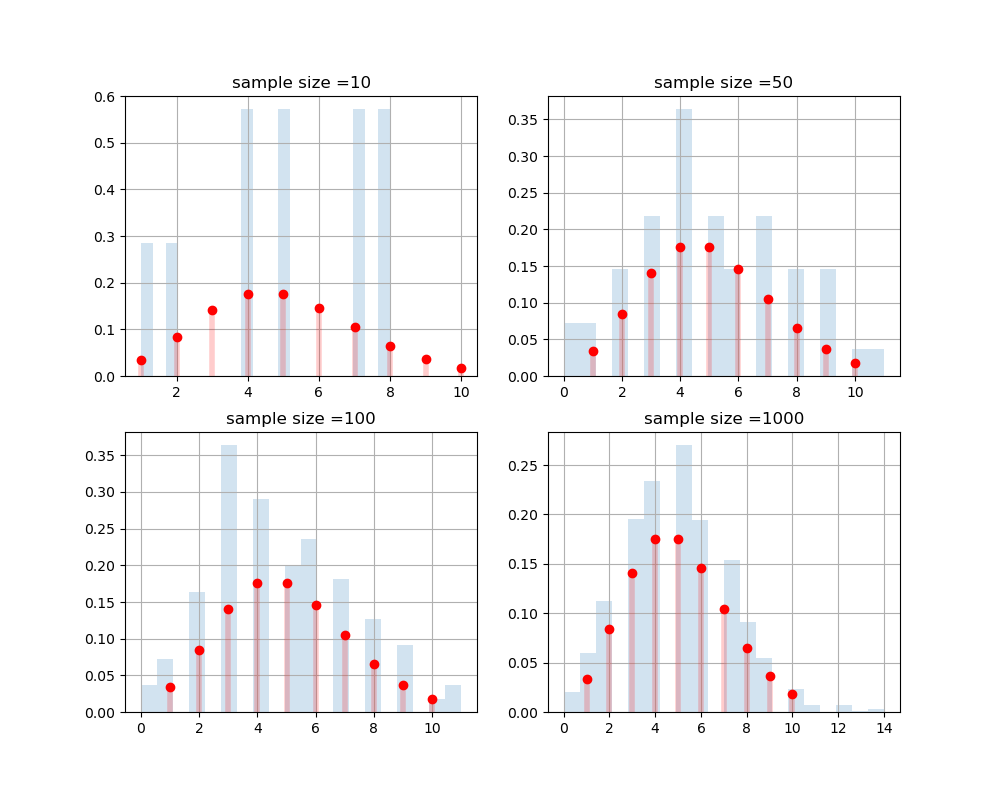
\includegraphics[width=\textwidth]{Lab1_poisson.png}
    \caption{Распределение Пуассона \eqref{eqn:poisson}}
    \label{fig:dis_pois_gis}
\end{figure}

\begin{figure}[H]
    \centering
    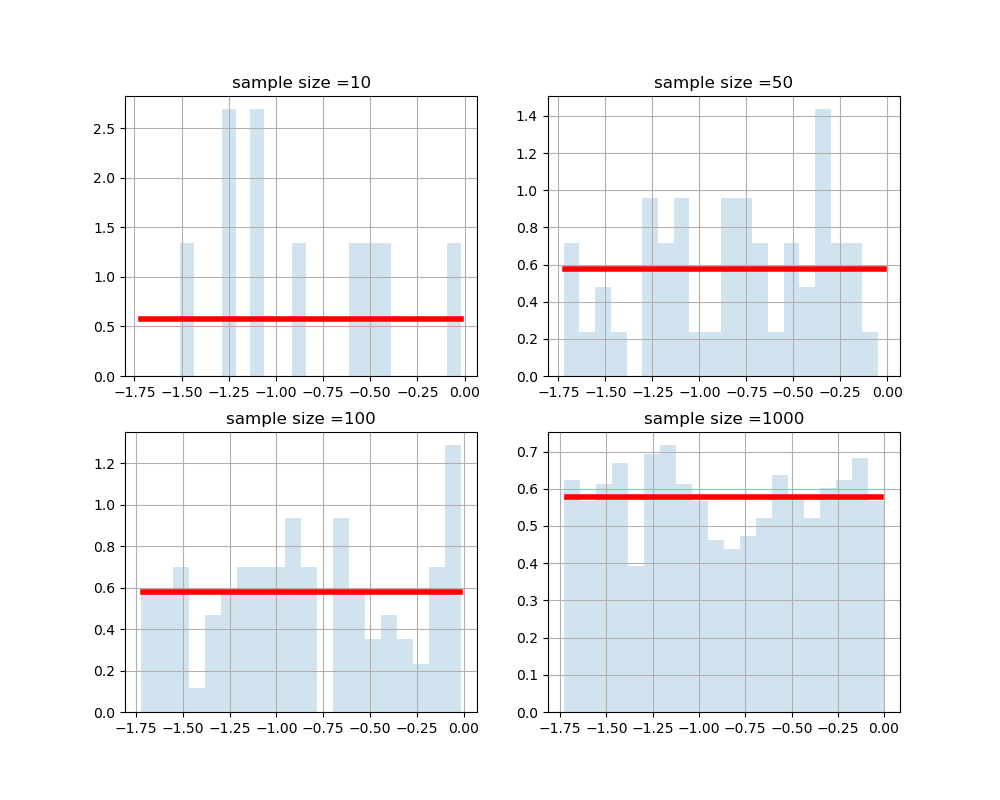
\includegraphics[width=\textwidth]{Lab1_uniform.png}
    \caption{Равномерное распределение \eqref{eqn:uniform}}
    \label{fig:dis_uni_gis}
\end{figure}


\subsection{Характеристики положения}
\begin{table}[H]
	\caption{\label{tab:normal} Стандартное нормальное распределение.}
	\begin{center}
		\begin{tabular}{|c|c|c|c|c|c|}
			\hline
			$n = 10$ & average & med & $Z_R$ & $Z_Q$ & $Z_{tr}$\\
			\hline
			$E =$ & $-0.0$ & $-0.02$ & $0.0$ & $-0.0$ & $-0.0$ \\
			\hline
			$D =$ & $0.106931$ & $0.145363$ & $0.186191$ & $0.111027$ & $0.165807$ \\
			\hline
			$n = 100$ & average & med & $Z_R$ & $Z_Q$ & $Z_{tr}$\\
			\hline
			$E =$ & $-0.0$ & $0.01$ & $0.02$ & $0.0$ & $0.0$\\
			\hline
			$D =$ & $0.010365$ &  $0.015172$ &  $0.092881$ &  $0.011974$ &  $0.017426$\\
			\hline
			$n = 1000$ & average & med & $Z_R$ & $Z_Q$ & $Z_{tr}$\\
			\hline
			$E =$ & $0.0$ & $0.0$ & $-0.0$ & $0.0$ & $0.0$\\
			\hline
			$D =$ & $0.00096$ &  $0.001594$ &  $0.060543$ &  $0.001256$ &  $0.001888$\\
			\hline
		\end{tabular}
	\end{center}
\end{table}

\begin{table}[H]
	\caption{\label{tab:cauchy} Стандартное распределение Лапласа.}
	\begin{center}
		\begin{tabular}{|c|c|c|c|c|c|}
			\hline
			$n = 10$   & average & med & $Z_R$ & $Z_Q$ & $Z_{tr}$\\ \hline
			$E =$ & $-0.01$ & $0.01$ &  $-0.0$ &  $-0.0$ &  $-0.01$\\ \hline
			$D =$  & $0.097868$ &  $0.069859$ &  $0.390201$ &  $0.093469$ &  $0.167235 $\\    \hline
			
			$n = 100$   & average & med & $Z_R$ & $Z_Q$ & $Z_{tr}$\\ \hline
			$E =$ &	$-0.0$ &  $0.01$ &  $0.01$ &  $0.0$ &  $-0.0$\\   \hline
			$D =$  & $0.009778$ &  $0.005878$ &  $0.429639$ &  $0.009072$ &  $0.020247$\\   \hline 
			
			$n = 1000$   & average & med & $Z_R$ & $Z_Q$ & $Z_{tr}$\\ \hline
			$E =$ & $0.0$ &  $0.0$ &  $-0.02$ &  $-0.0$ &  $0.0$\\  \hline
			$D =$ & $0.001009$ &  $0.000531$ &  $0.428975$ &  $0.000997$ &  $0.001992$\\    
			\hline
		\end{tabular}
	\end{center}
\end{table}

\begin{table}[H]
	\caption{\label{tab:laplace} Распределение Коши.}
	\begin{center}
		\begin{tabular}{|c|c|c|c|c|c|}
			\hline
			$n = 10$    & average & med & $Z_R$ & $Z_Q$ & $Z_{tr}$\\ \hline 
			$E = $  & $0.31$ &  $-0.01$ &  $-5.87$ &  $0.03$ &  $3.5$\\ \hline
			$D = $  & $260.978036$ &  $0.347366$ &  $26462.674037$ &  $0.774488$ &  $6529.2454$\\ \hline
			
			$n = 100$  & average & med & $Z_R$ & $Z_Q$ & $Z_{tr}$\\ \hline
			$E = $ & $2.26$ &  $0.01$ &  $22.79$ &  $-0.0$ &  $1.71$   \\ \hline
			$D =$ & $2122.106445$ &  $0.023531$ &  $1741103.211025$ &  $0.05289$ &  $1778.363557$    \\ \hline
			
			$n = 1000$   & average & med & $Z_R$ & $Z_Q$ & $Z_{tr}$\\ \hline
			$E =$ & $1.14$ &  $0.0$ &  $-1845.52$ &  $-0.0$ &  $-1.64$   \\ \hline
			$D = $ & $706.431432$ &  $0.002497$ &  $21117320297.542297$ &  $0.004864$ &  $1675.403679$    \\ 
			\hline
		\end{tabular}
	\end{center}
\end{table}

\begin{table}[H]
	\caption{\label{tab:uniform} Равномерное распределение.}
	\begin{center}
		\begin{tabular}{|c|c|c|c|c|c|}
			\hline
			$n = 10$  & average & med & $Z_R$ & $Z_Q$ & $Z_{tr}$\\ \hline
			$E =$ &	$-0.02$  & 	$0.0$  & 	$0.0$    &	$-0.0$   &	$-0.02$  \\ \hline  
			$D =$ &	$0.095612$  &  $0.227685$  &  $0.043735$  &  $0.135551$  &  $0.171826$    \\ \hline
			
			$n = 100$  & average & med & $Z_R$ & $Z_Q$ & $Z_{tr}$\\ \hline
			$E =$  &	$0.0$   & 	$-0.0$   &	$-0.0$   &	$0.0$   & 	$0.01$    \\ \hline
			$D =$ &	$0.009971$   &  $0.029194$   &  $0.00058$   &  $0.014725$   &  $0.019723$  \\ \hline
			
			$n = 1000$  & average & med & $Z_R$ & $Z_Q$ & $Z_{tr}$\\ \hline
			$E =$  &  	$-0.0$    &	$0.0$    &	$-0.0 $  & 	$0.0$   & 	$-0.0$    \\ \hline
			$D =$ & $0.000959$   &  $0.002864$   &  $6e-06$   &  $0.001502$   &  $0.00205$    \\
			\hline
		\end{tabular}
	\end{center}
\end{table}

\begin{table}[H]
	\caption{\label{tab:poisson} Распределение Пуассона.}
	\begin{center}
		\begin{tabular}{|c|c|c|c|c|c|}
			\hline
			$n = 10$   & average & med & $Z_R$ & $Z_Q$ & $Z_{tr}$\\ \hline
			$E =$ & $5.01$ &  $4.84$ &  $5.3$ &  $4.88$ &  $5.02$    \\ \hline
			$D =$ & $0.515302$ &  $0.739579$ &  $0.942244$ &  $0.586539$ &  $0.832244$    \\ \hline
			
			$n = 100$   & average & med & $Z_R$ & $Z_Q$ & $Z_{tr}$\\ \hline
			$E =$ & $5.0$ &  $4.9$ &  $5.97$ &  $4.89$ &  $4.99$ \\ \hline
			$D =$ &	$0.049874$ &  $0.102596$ &  $0.499128$ &  $0.143341$ &  $0.101492$ \\ \hline
			
			$n = 1000$   & average & med & $Z_R$ & $Z_Q$ & $Z_{tr}$\\ \hline
			$E =$ & $5.0$ &  $5.0$ &  $6.83$ &  $4.67$ &  $5.0$    \\ \hline
			$D =$ & $0.005329$ &  $0.0$ &  $0.341759$ &  $0.076798$ &  $0.010249$    \\
			\hline
		\end{tabular}
	\end{center}
\end{table}


\subsection{Боксплот Тьюки}
\begin{center}
	
	\begin{figure}[H]
		\caption{Boxplot распределений для размера выборки N=20 }
		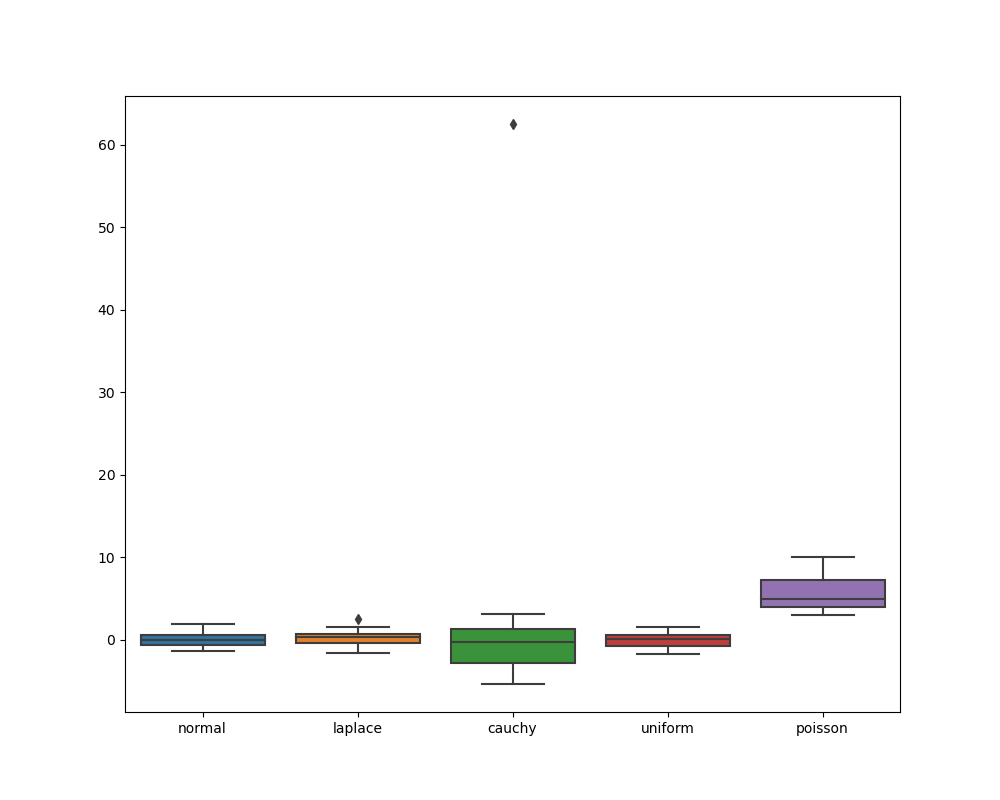
\includegraphics[width=\textwidth]{Lab3_boxplot_N=20.png}
	\end{figure}
	
	\begin{figure}[H]
		\caption{Boxplot стандартное нормальное распределение }
		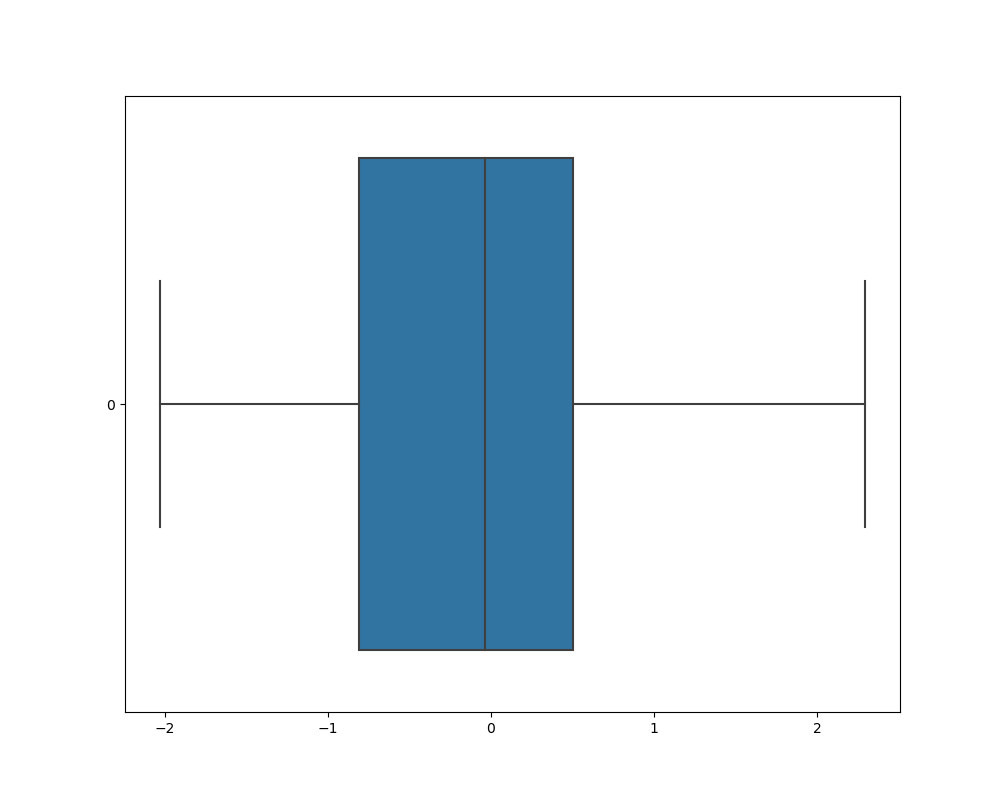
\includegraphics[width=\textwidth]{Lab3_boxplot_N=100_normal.png} 
	\end{figure}
	
	\begin{figure}[H]
		\caption{Boxplot стандартное распределение Лапласа }
		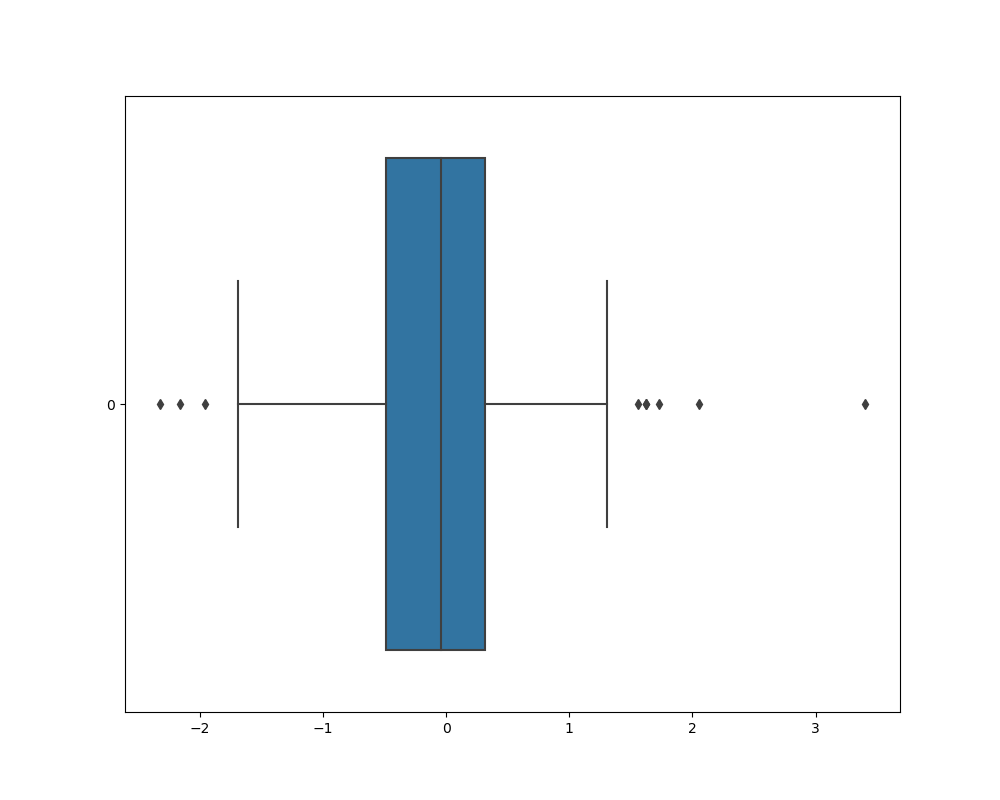
\includegraphics[width=\textwidth]{Lab3_boxplot_N=100_laplace.png} 
	\end{figure}
	
	\begin{figure}[H]
		\caption{Boxplot стандартное распределение Коши }
		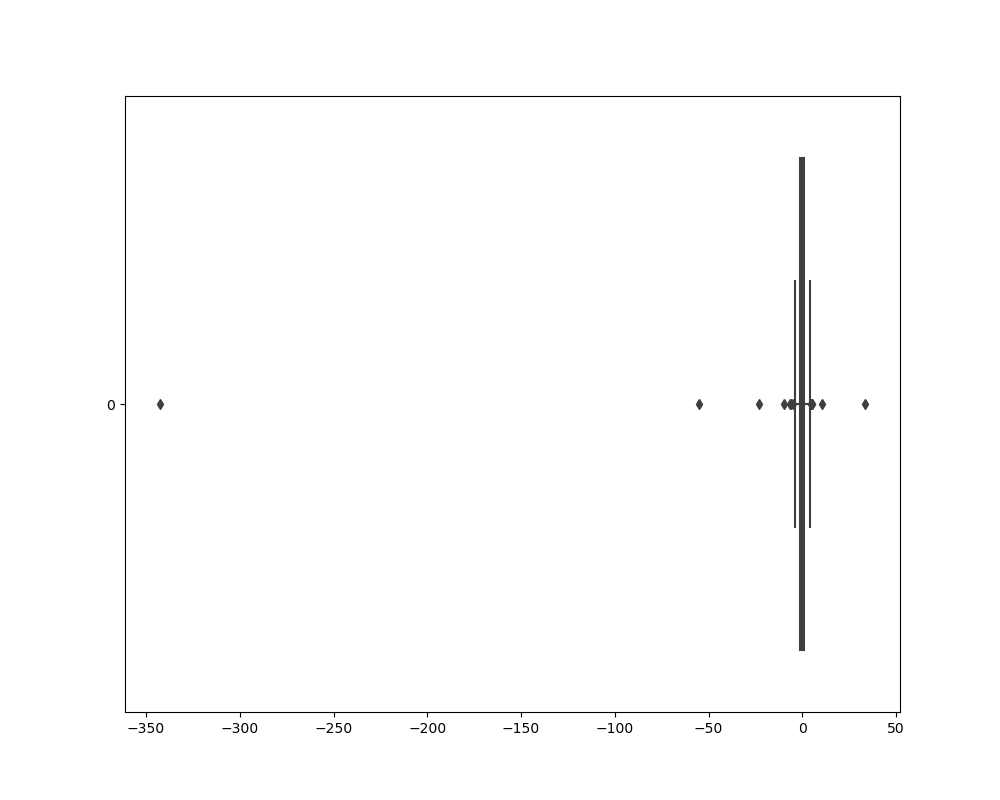
\includegraphics[width=\textwidth]{Lab3_boxplot_N=100_cauchy.png} 
	\end{figure}
	
	\begin{figure}[H]
		\caption{Boxplot распределение Пуассона }
		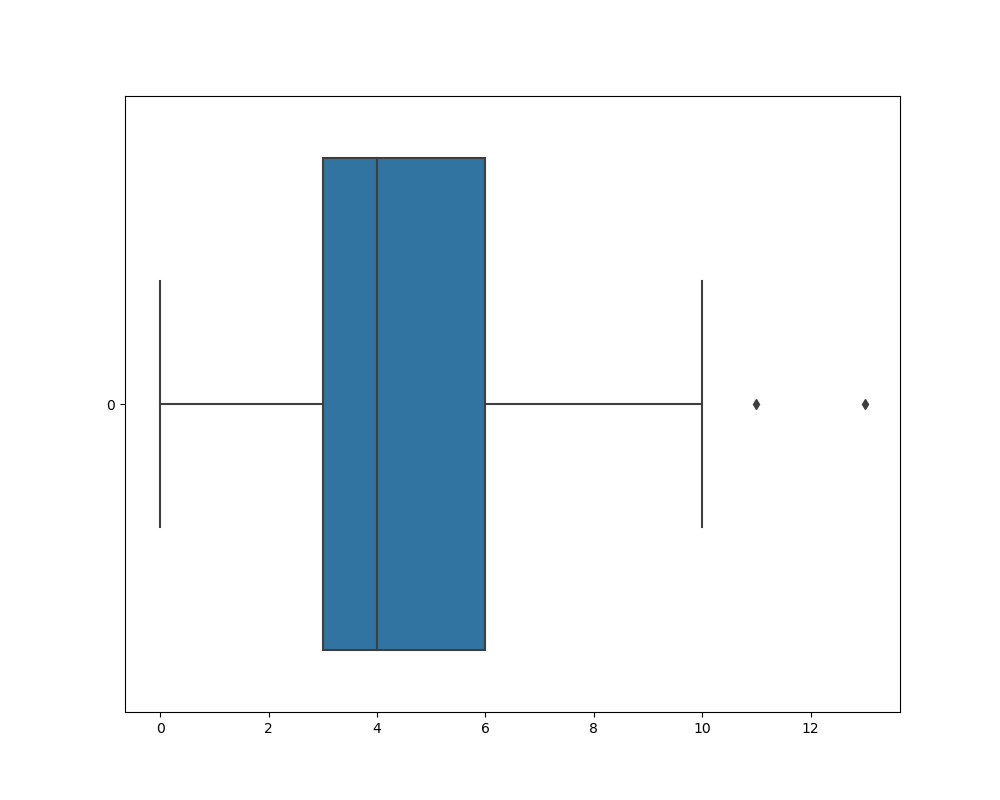
\includegraphics[width=\textwidth]{Lab3_boxplot_N=100_poisson.png} 
	\end{figure}
	
	\begin{figure}[H]
		\caption{Boxplot равномерное распределение }
		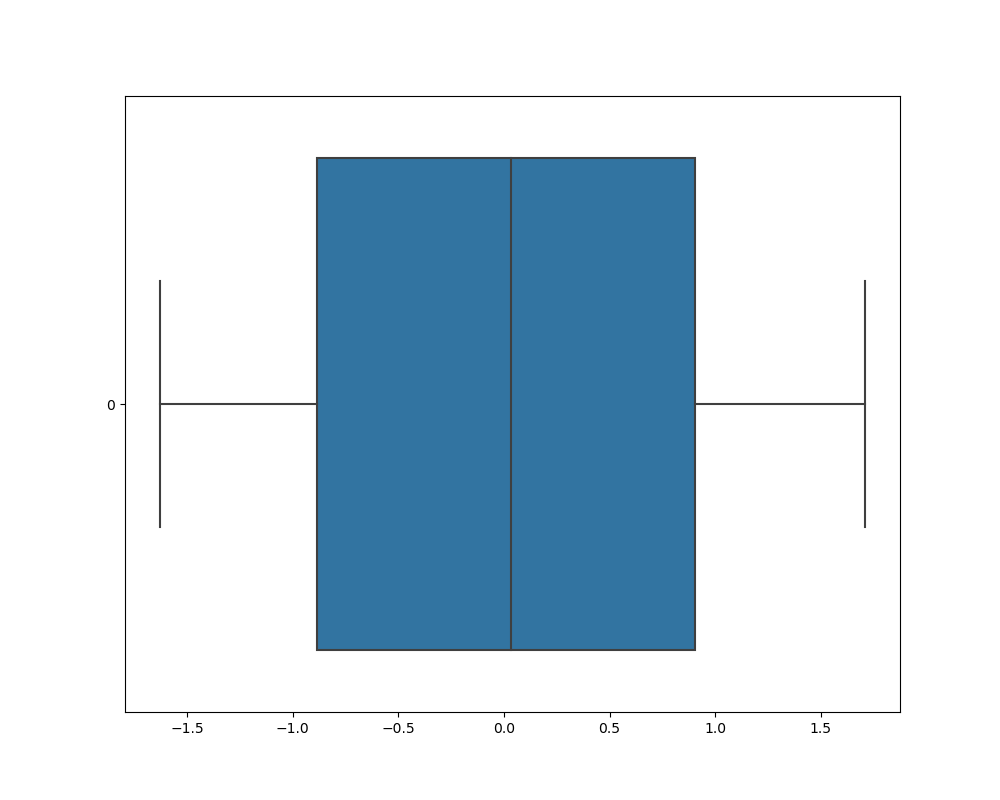
\includegraphics[width=\textwidth]{Lab3_boxplot_N=100_uniform.png}
	\end{figure}
	
	\begin{table}[H]
		
		\caption{Теоретические оценки доли выбрасов}
		\label{tab:my_label}
		\begin{center}
			\vspace{5mm}
			\begin{tabular}{|c|c|}
				\hline
				Распределение & Доля выбросов\\
				\hline
				normal	& $0.006977$\\
				\hline
				cauchy & $0.155958$\\
				\hline
				laplace	& $0.0625$\\
				\hline
				uniform	& $0.0$\\
				\hline
				poisson	& $0.013695$\\
				\hline
			\end{tabular}
			
		\end{center}
		
	\end{table}
	
	\begin{table}[H]
		
		\caption{Экспериментальные оценки доли выбросов}
		\label{tab:my_label}
		\begin{center}
			\vspace{5mm}
			\begin{tabular}{|c|c|c|}
				\hline
				Распределение & Средняя доля выбросов & Дисперсия доли выбросов\\
				\hline
				normal	& &\\
				\hline
				n = 20   & 	$0.02$ &  $ 0.00152 $ \\
				\hline
				n = 100   &	$0.01$ & $ 0.000161 $   \\
				\hline
				cauchy	& &\\
				\hline
				n = 20   & 	$0.15$ & $ 0.004827 $   \\
				\hline
				n = 100  & 	$0.155$  & $ 0.001067 $  \\
				\hline
				laplace	& &\\
				\hline
				n = 20    &	$0.07$  & $ 0.004469 $  \\
				\hline
				n = 100   &	$0.065$ & $ 0.000995 $   \\
				\hline
				uniform	& &\\
				\hline
				n = 20    &	$0.002$ & $ 0.000212 $   \\
				\hline
				n = 100   &	$0.0$ & $ 0.0 $  \\ 
				\hline
				poisson	& &\\
				\hline
				n = 20   & 	$0.02$ & $ 0.002284 $   \\
				\hline
				n = 100  & 	$0.014$ & $ 0.000285 $   \\
				\hline
			\end{tabular}
			
		\end{center}
		
	\end{table}
	
\end{center}

\subsection{Ядерные функции}
\begin{center}
	
	\begin{figure}[H]
		\caption{Ядерная функция плотности для нормального распределения n = $20$ }
		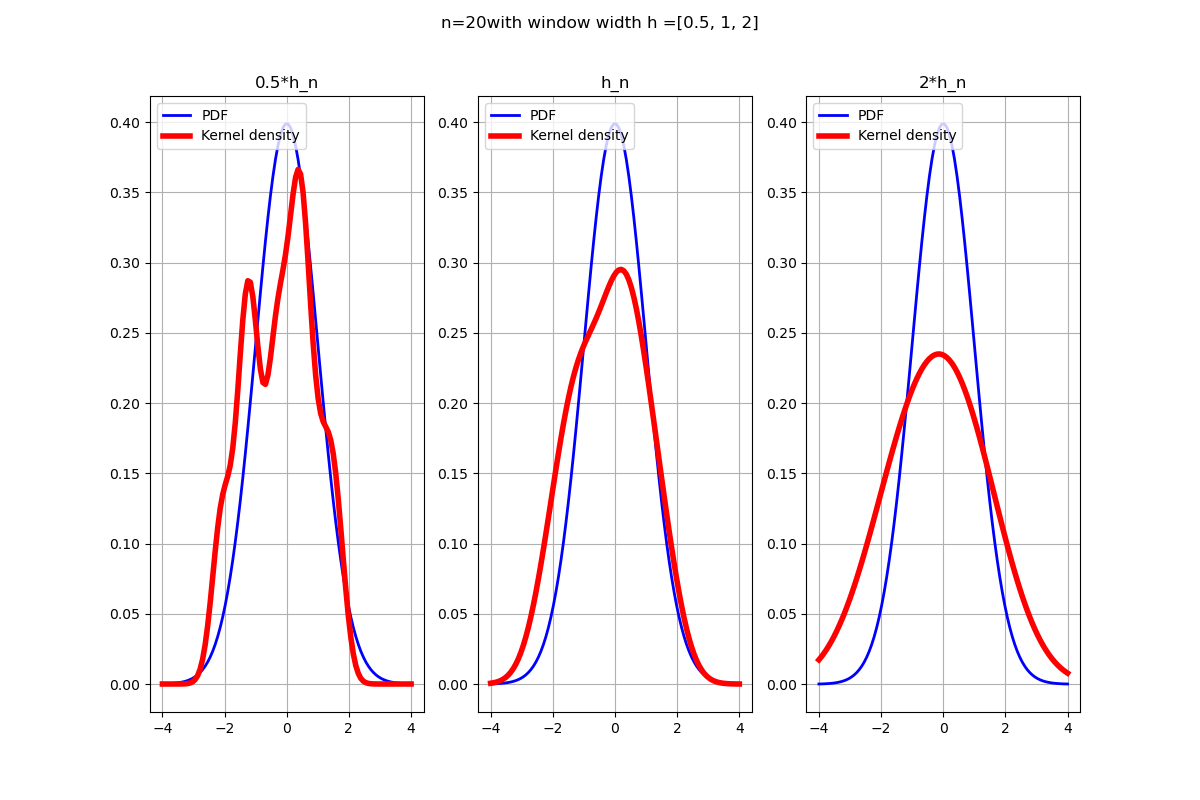
\includegraphics[width=\textwidth]{Lab4_normal_pdf_20.png}
	\end{figure}
	
	\begin{figure}[H]
		\caption{Ядерная функция плотности для нормального распределения n = $60$ }
		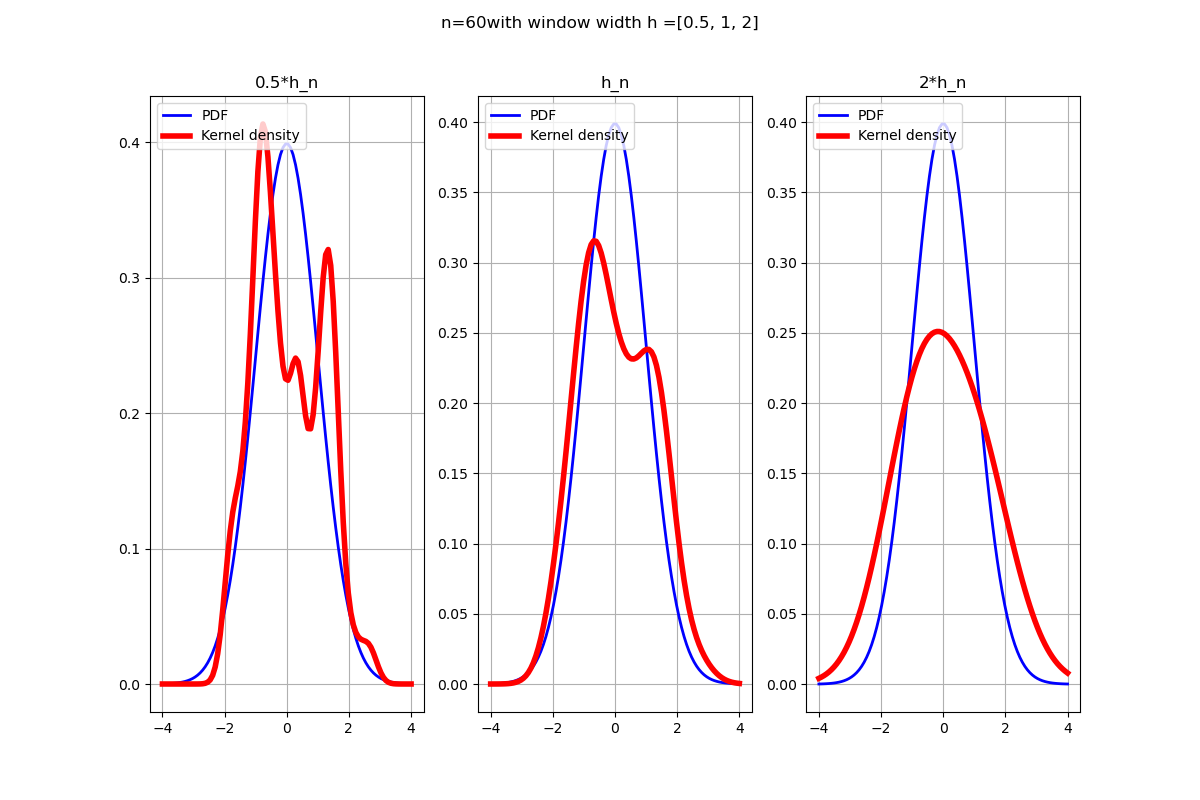
\includegraphics[width=\textwidth]{Lab4_normal_pdf_60.png}
	\end{figure}
	
	\begin{figure}[H]
		\caption{Ядерная функция плотности для нормального распределения n = $100$ }
		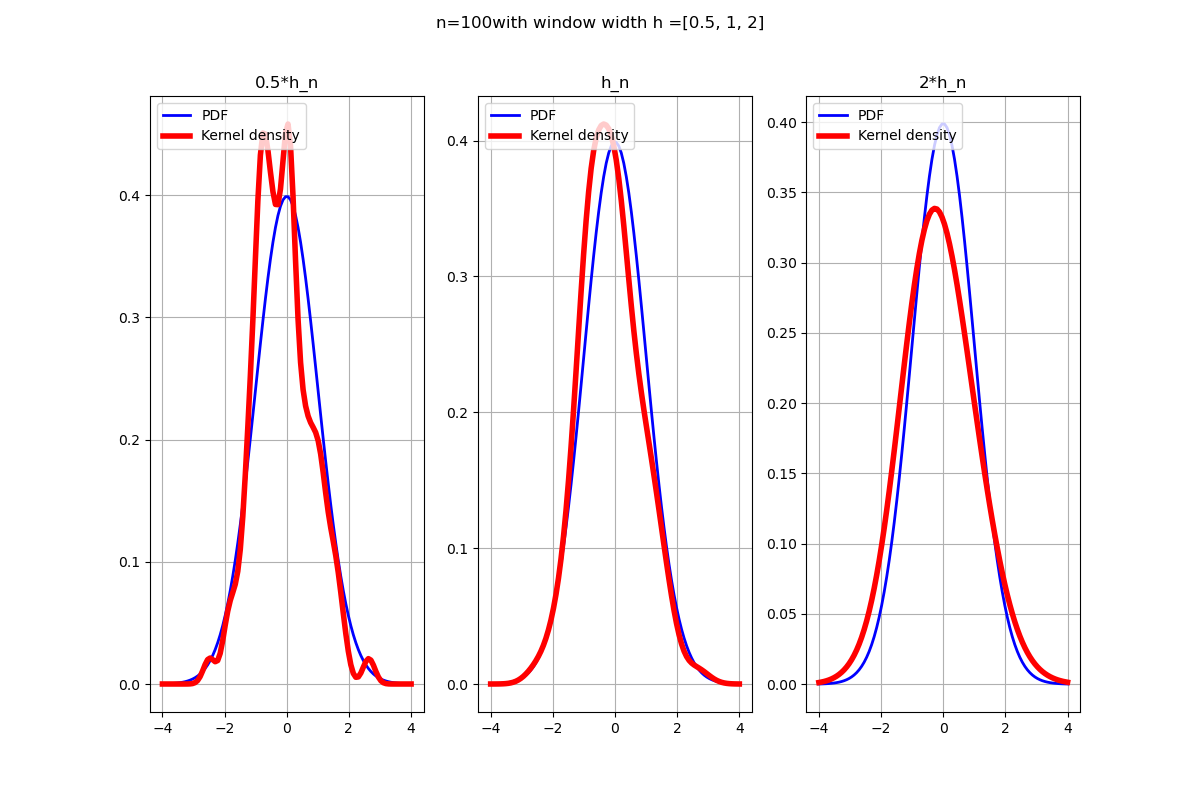
\includegraphics[width=\textwidth]{Lab4_normal_pdf_100.png}
	\end{figure}
	
	\begin{figure}[H]
		\caption{Ядерная функция плотности для распределения Лапласа n = $20$ }
		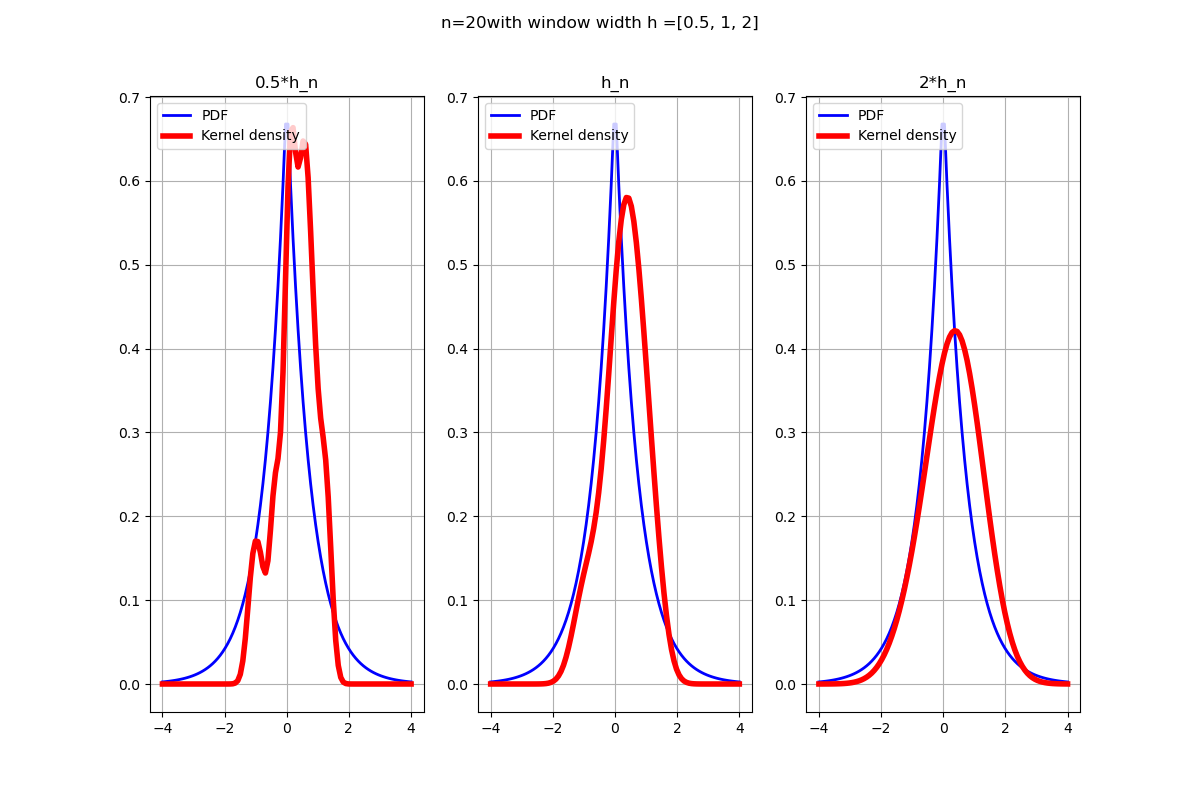
\includegraphics[width=\textwidth]{Lab4_laplace_pdf_20.png} 
	\end{figure}
	
	\begin{figure}[H]
		\caption{Ядерная функция плотности для распределения Лапласа n = $60$ }
		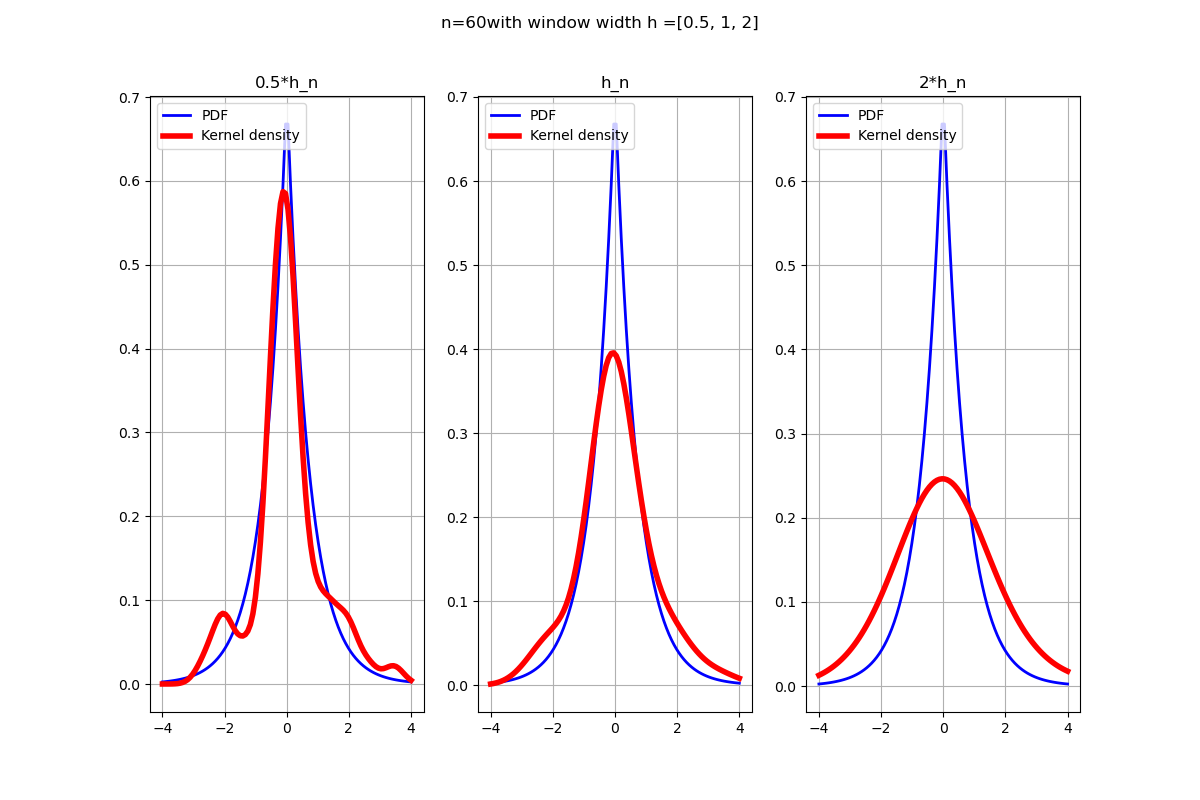
\includegraphics[width=\textwidth]{Lab4_laplace_pdf_60.png} 
	\end{figure}
	
	\begin{figure}[H]
		\caption{Ядерная функция плотности для распределения Лапласа n = $100$ }
		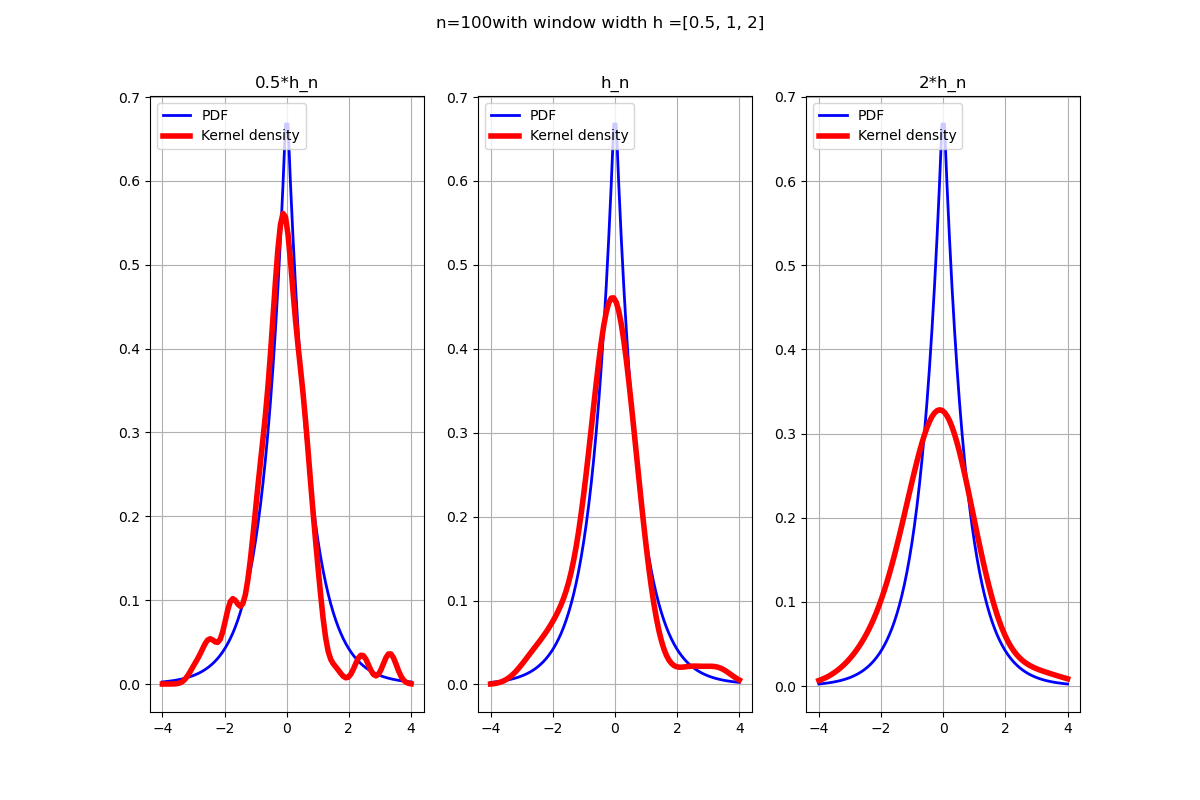
\includegraphics[width=\textwidth]{Lab4_laplace_pdf_100.png} 
	\end{figure}
	
	\begin{figure}[H]
		\caption{Ядерная функция плотности для распределения Коши n = $20$ }
		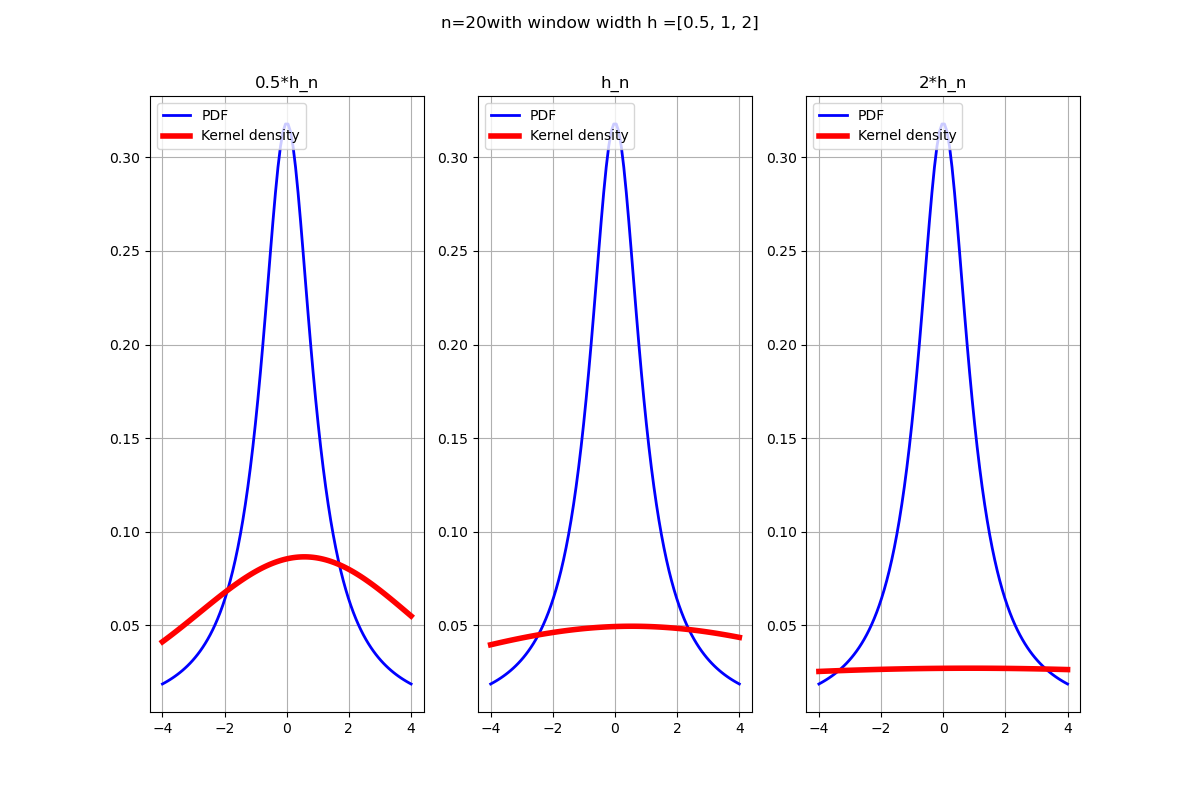
\includegraphics[width=\textwidth]{Lab4_cauchy_pdf_20.png} 
	\end{figure}
	
	\begin{figure}[H]
		\caption{Ядерная функция плотности для распределения Коши n = $60$ }
		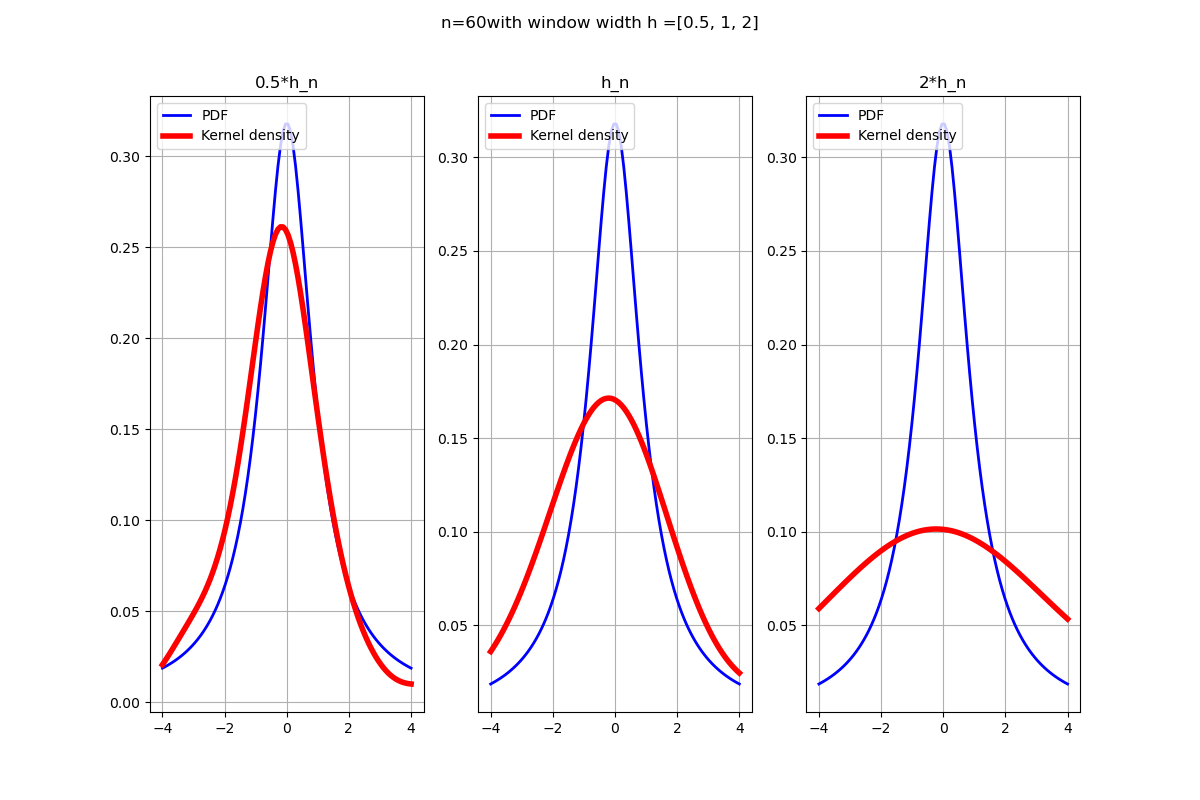
\includegraphics[width=\textwidth]{Lab4_cauchy_pdf_60.png} 
	\end{figure}
	
	\begin{figure}[H]
		\caption{Ядерная функция плотности для распределения Коши n = $100$ }
		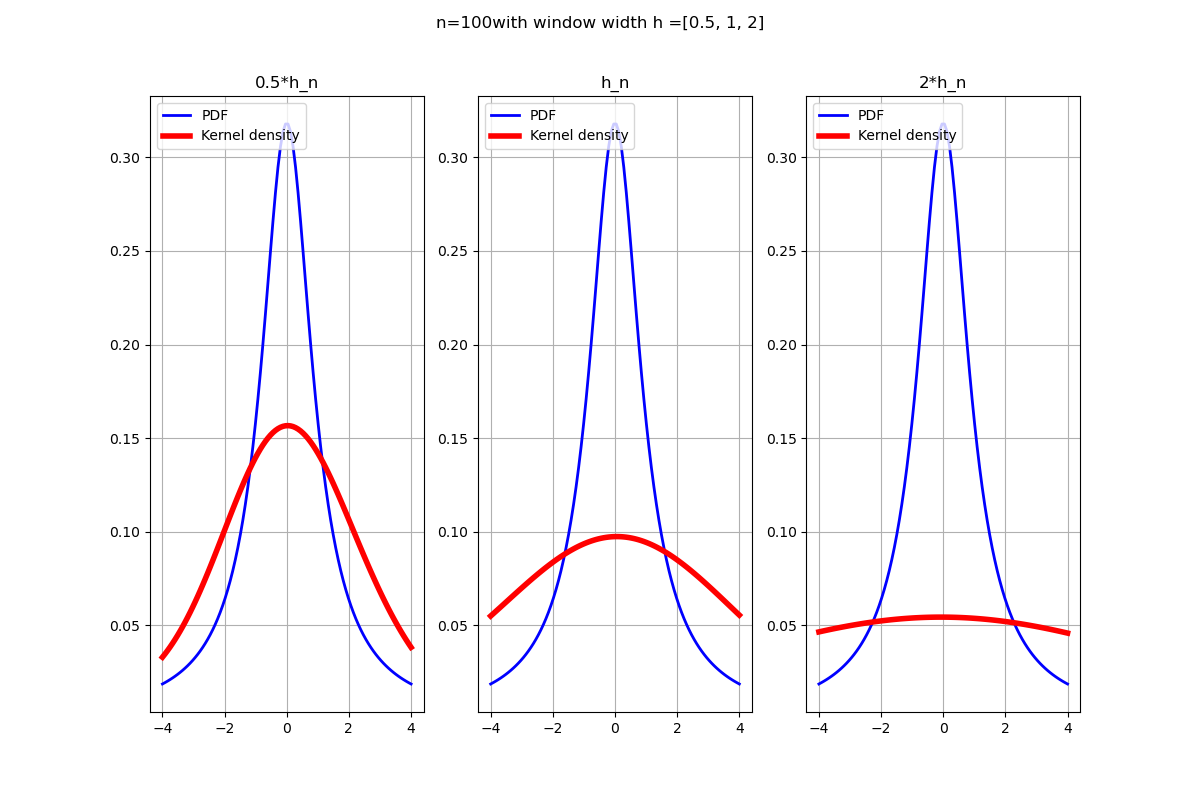
\includegraphics[width=\textwidth]{Lab4_cauchy_pdf_100.png} 
	\end{figure}
	
	\begin{figure}[H]
		\caption{Ядерная функция плотности для распределения Пуассона n = $20$}
		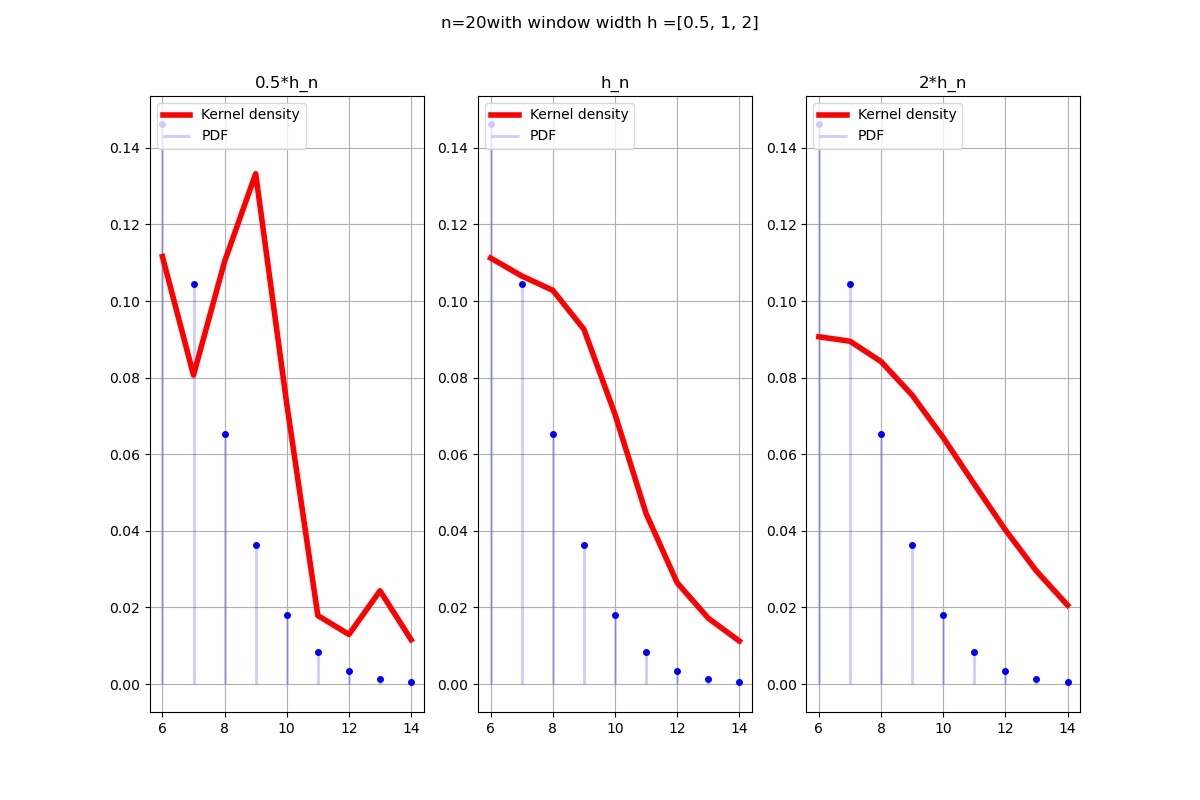
\includegraphics[width=\textwidth]{Lab4_poisson_pdf_20.png} 
	\end{figure}
	
	\begin{figure}[H]
		\caption{Ядерная функция плотности для распределения Пуассона n = $60$}
		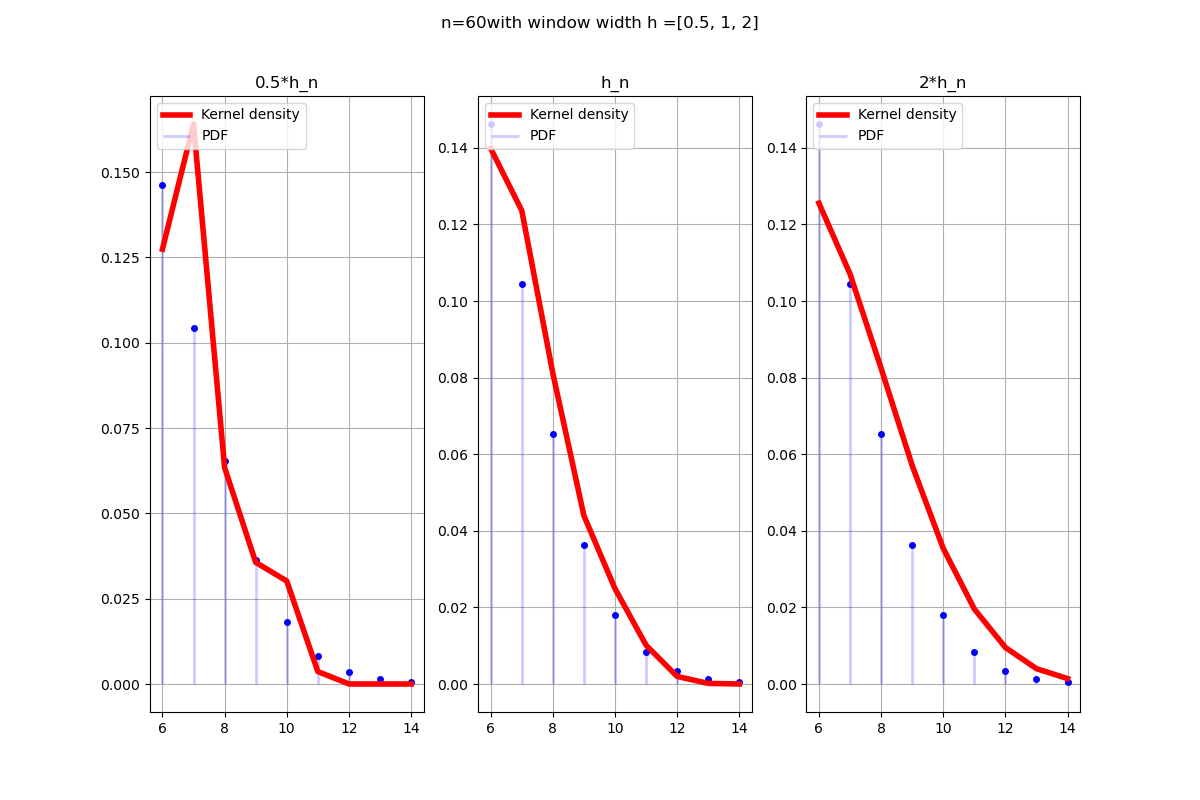
\includegraphics[width=\textwidth]{Lab4_poisson_pdf_60.png} 
	\end{figure}
	
	\begin{figure}[H]
		\caption{Ядерная функция плотности для распределения Пуассона n = $100$}
		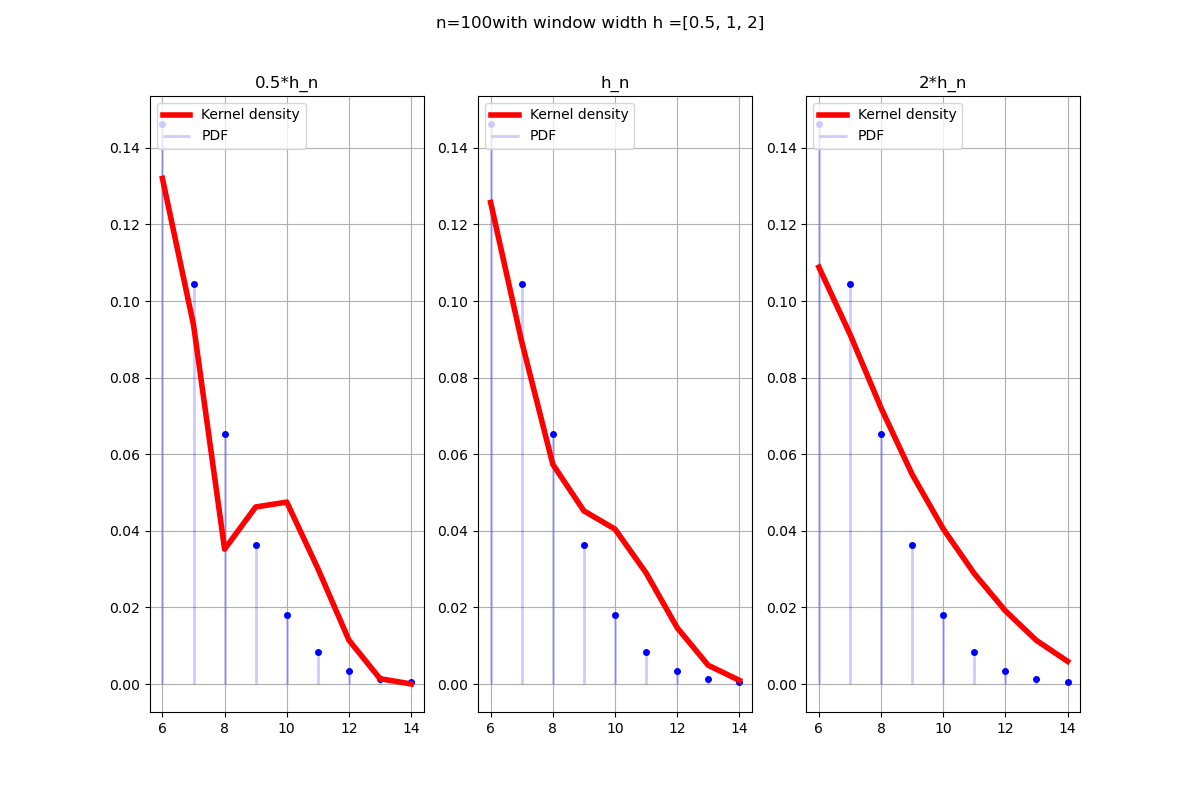
\includegraphics[width=\textwidth]{Lab4_poisson_pdf_100.png} 
	\end{figure}
	
	\begin{figure}[H]
		\caption{ Ядерная функция плотности для равномерного распределения n = $20$}
		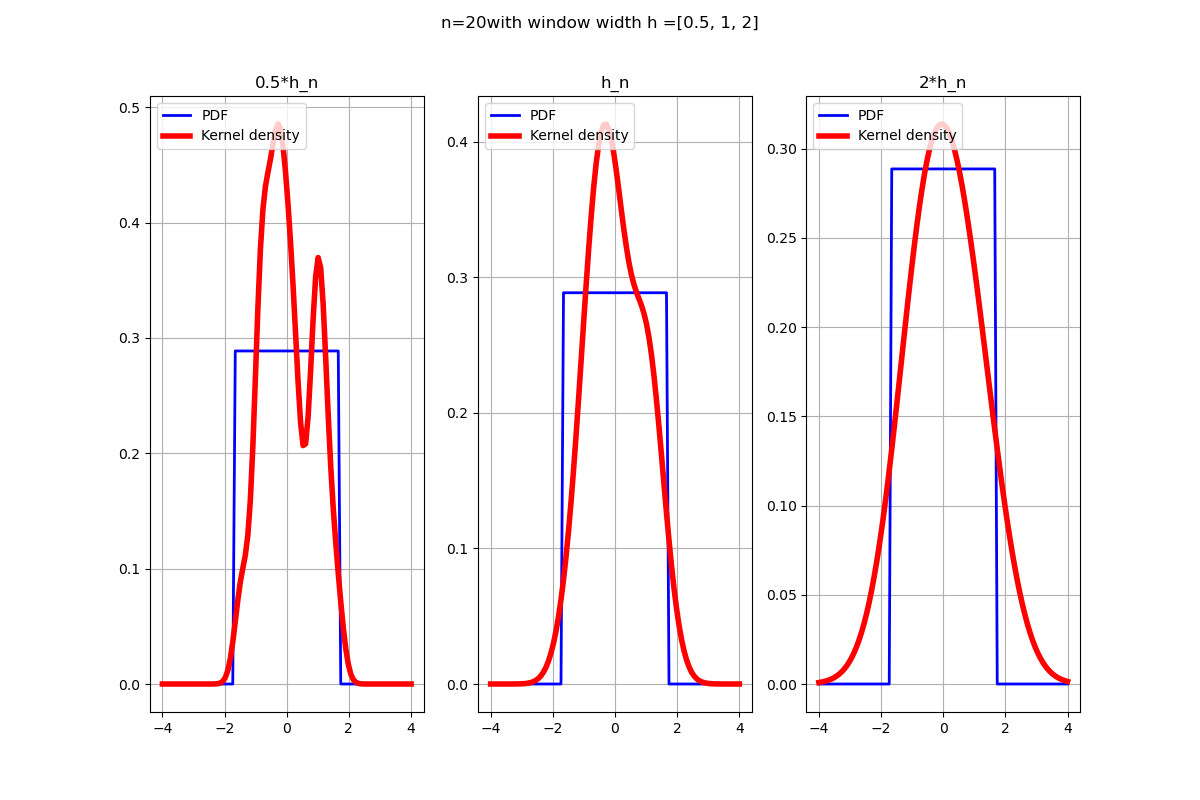
\includegraphics[width=\textwidth]{Lab4_uniform_pdf_20.png} 
	\end{figure}
	
	\begin{figure}[H]
		\caption{ Ядерная функция плотности для равномерного распределения n = $60$}
		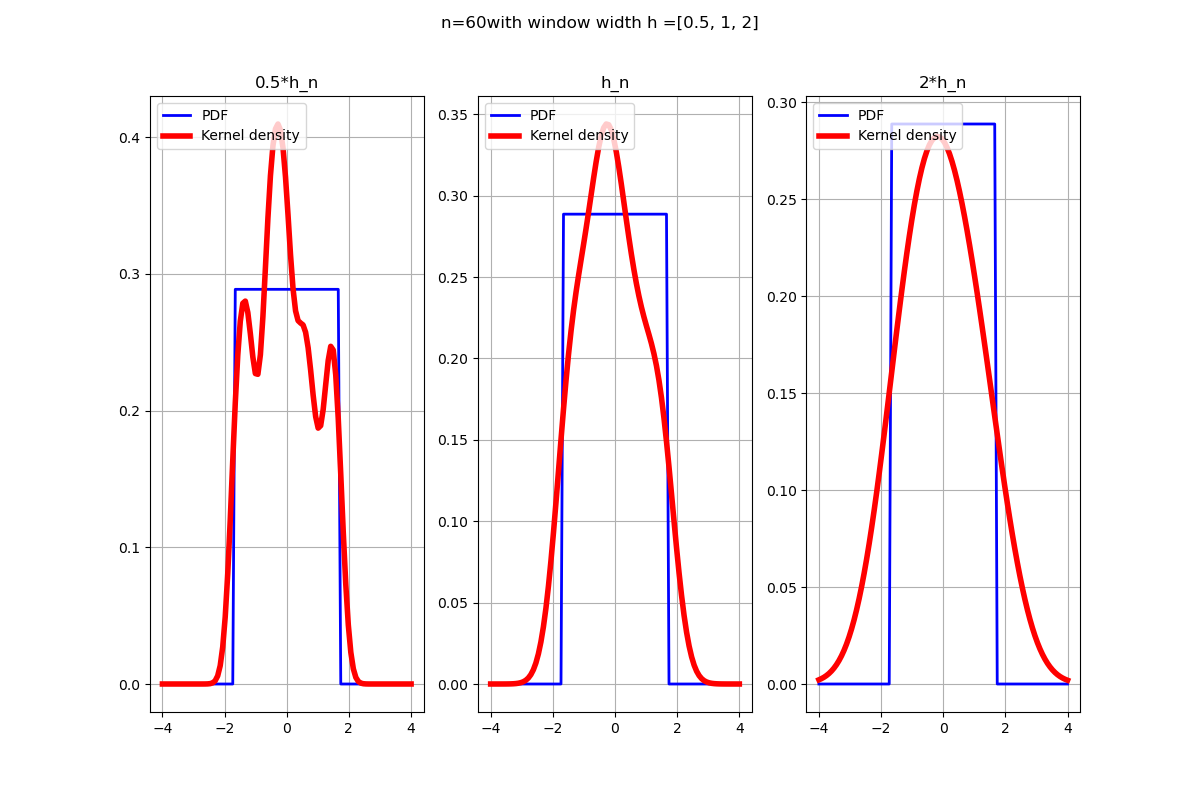
\includegraphics[width=\textwidth]{Lab4_uniform_pdf_60.png} 
	\end{figure}
	
	\begin{figure}[H]
		\caption{ Ядерная функция плотности для равномерного распределения n = $100$}
		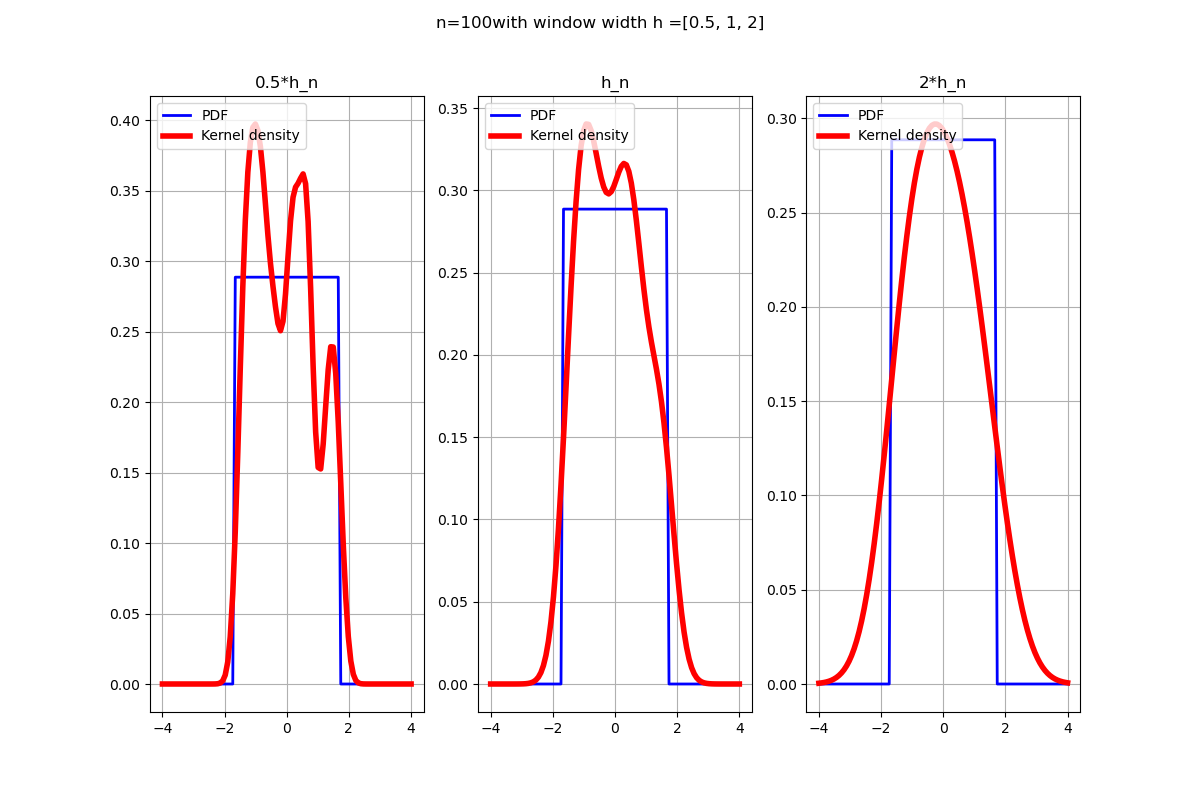
\includegraphics[width=\textwidth]{Lab4_uniform_pdf_100.png} 
	\end{figure}
	
\end{center}
\subsection{Эмпирические функции распределения}
\begin{center}
	\begin{figure}[H]
		\caption{Эмпирическая функция для стандартного нормального распределения}
		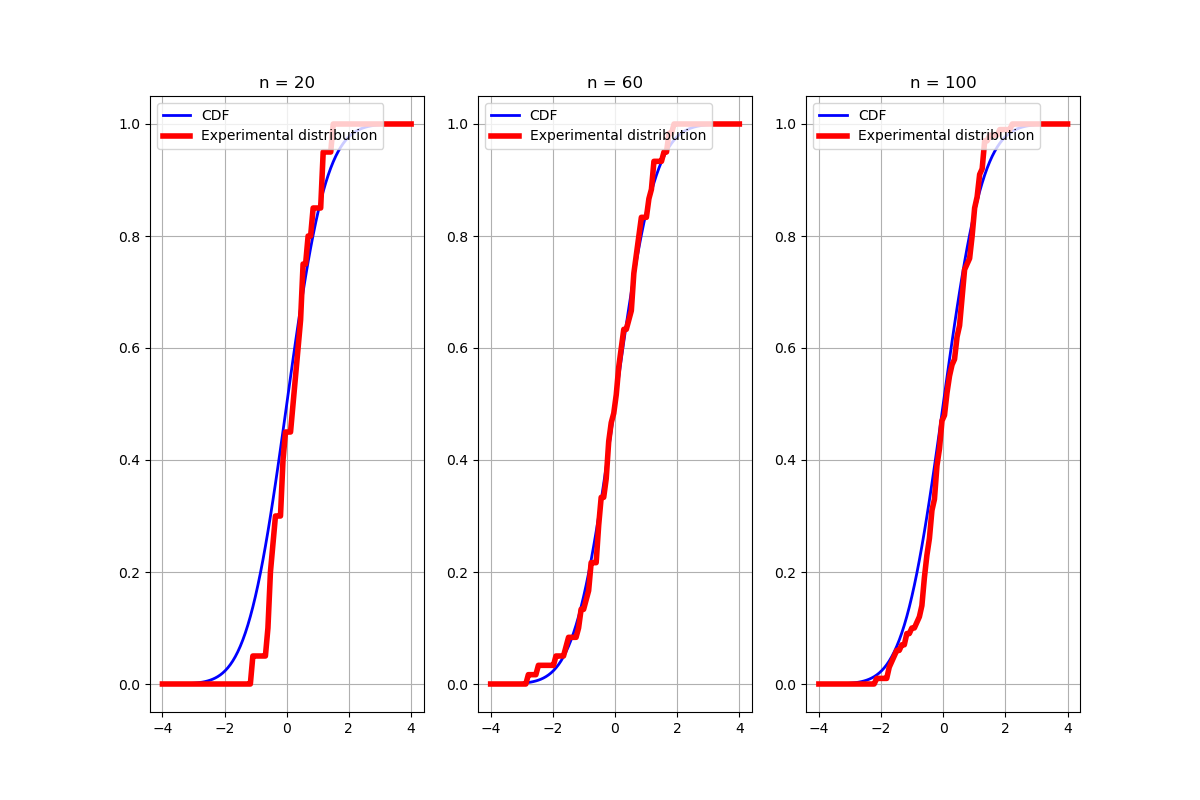
\includegraphics[width=\textwidth]{Lab4_normal_cdf.png}
	\end{figure}
	\begin{figure}[H]
		\caption{Эмпирическая функция для стандартного распределения Лапласа}
		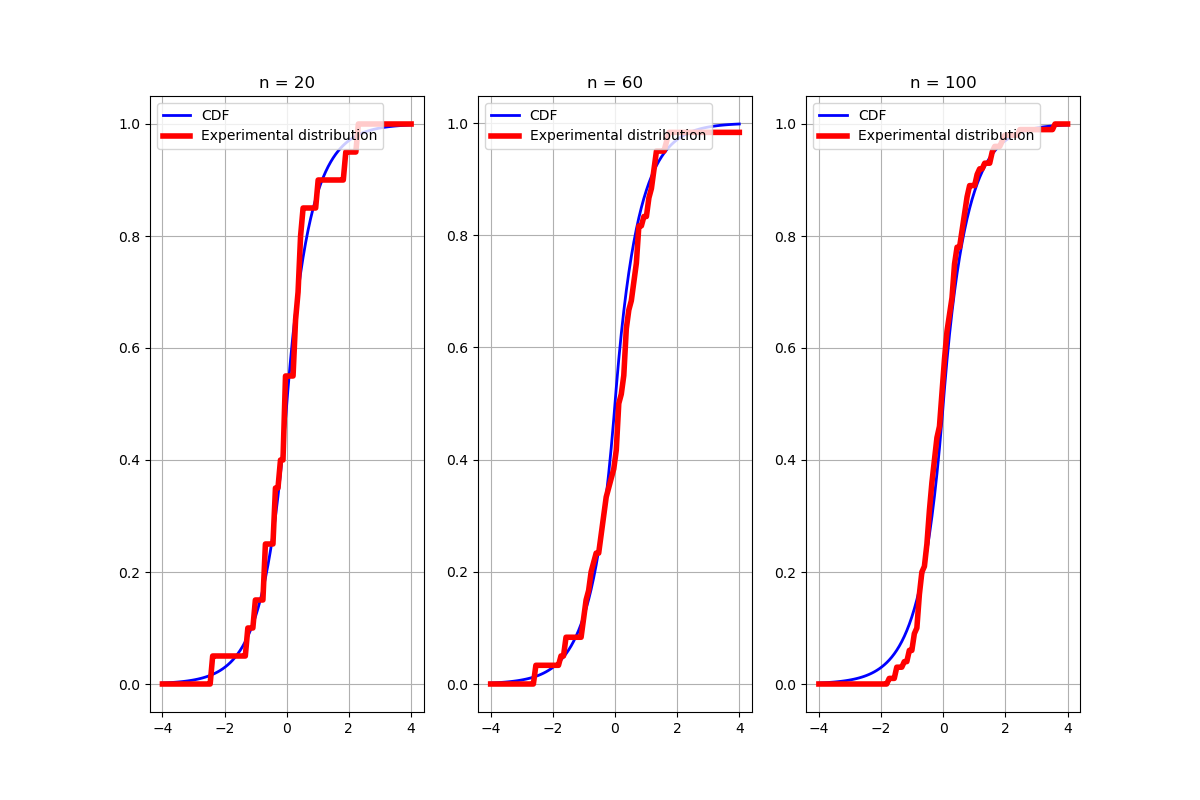
\includegraphics[width=\textwidth]{Lab4_laplace_cdf.png}
	\end{figure}
	\begin{figure}[H]
		\caption{Эмпирическая функция для стандартного распределения Коши}
		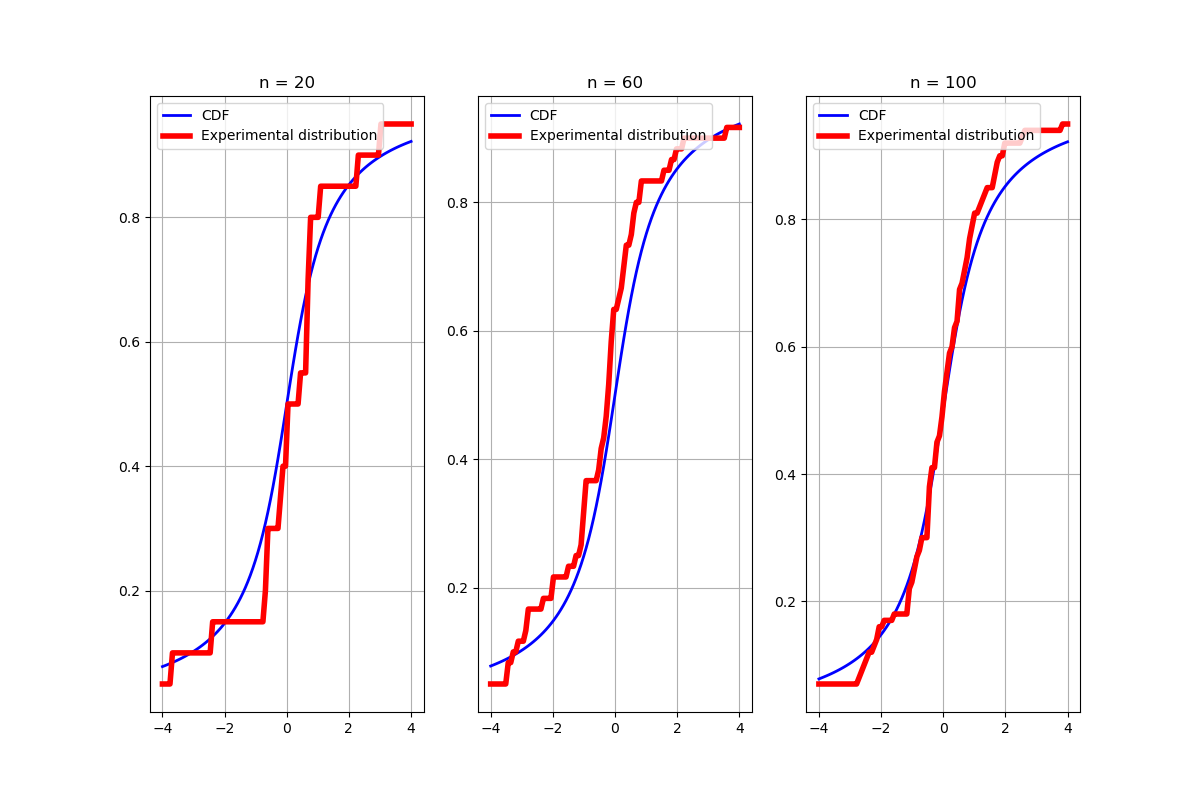
\includegraphics[width=\textwidth]{Lab4_cauchy_cdf.png}
	\end{figure}
	\begin{figure}[H]
		\caption{Эмпирическая функция для распределения Пуассона}
		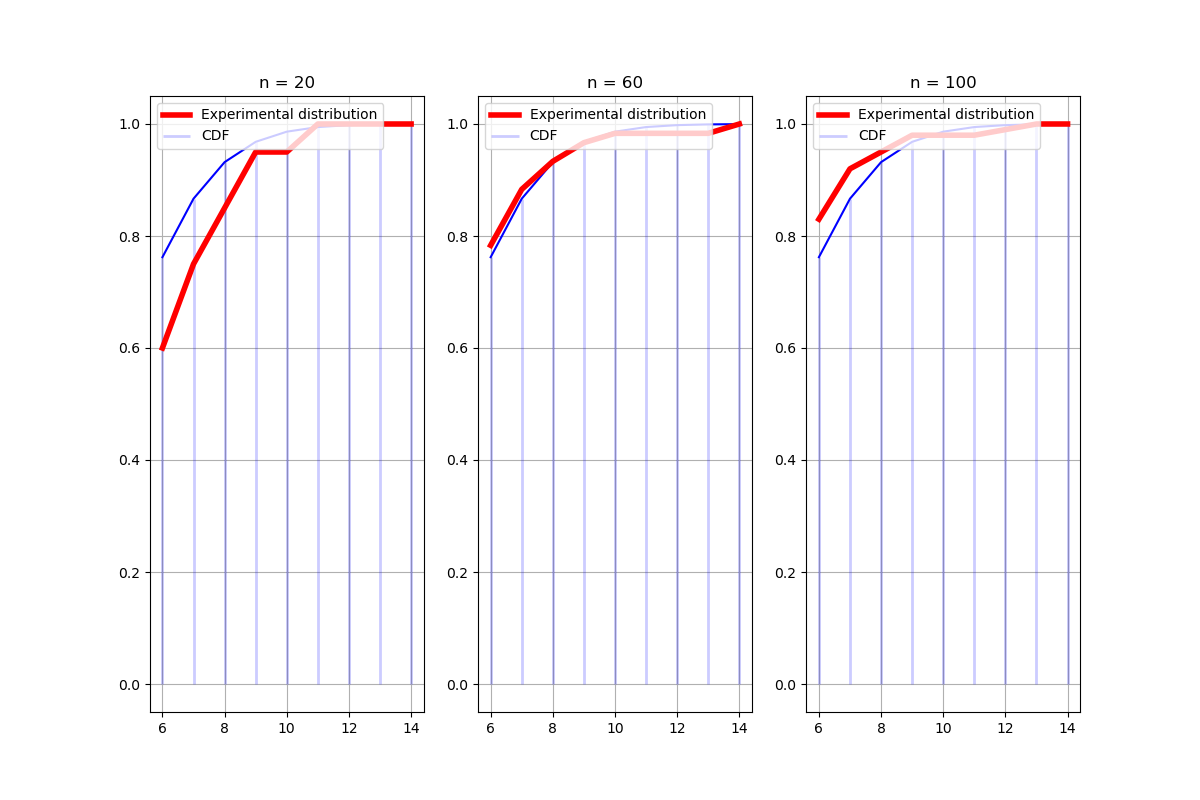
\includegraphics[width=\textwidth]{Lab4_poisson_cdf.png}
	\end{figure}
	\begin{figure}[H]
		\caption{Эмпирическая функция для равномерного распределения}
		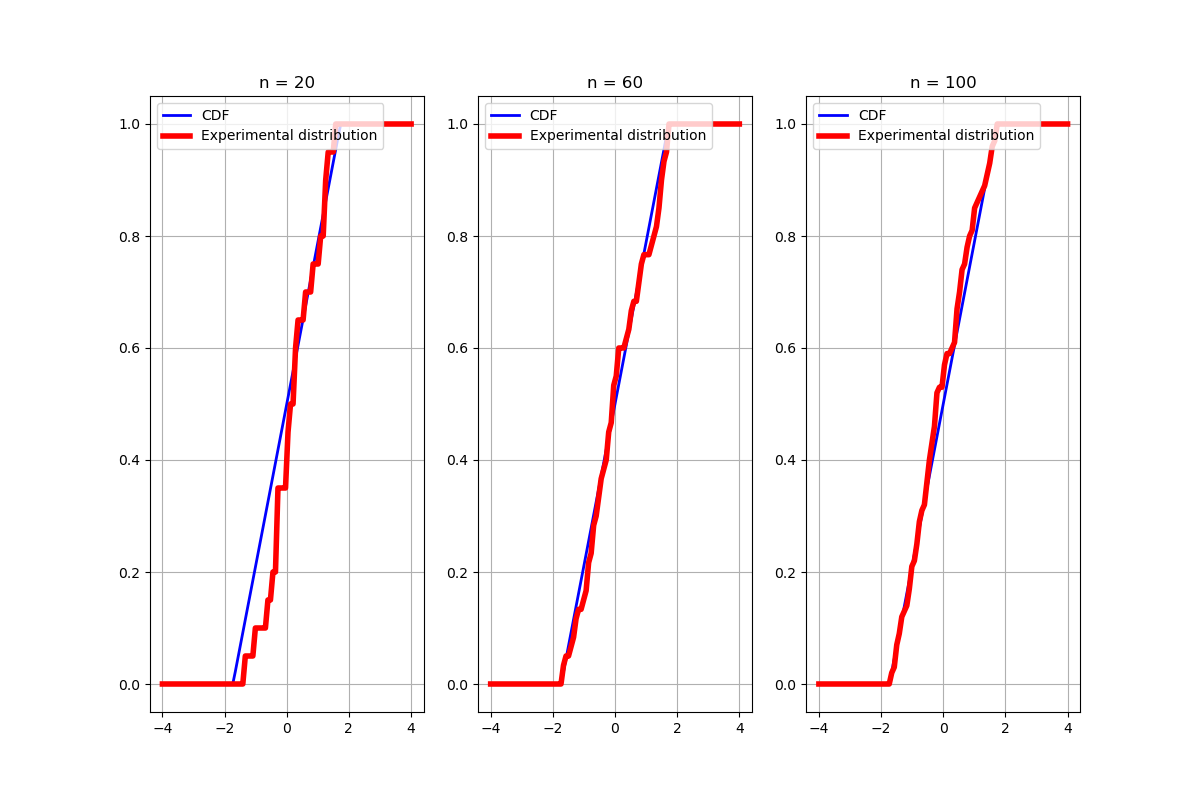
\includegraphics[width=\textwidth]{Lab4_uniform_cdf.png}
	\end{figure}
\end{center}
\section{Обсуждение}
\subsection{Характеристики положения}
\par При вычислении средних значений пришлось отбрасывать некоторое число знаков после запятой, так как получаемая дисперсия не могла гарантировать получаемое точное значение. \par Иными словами дисперсия может гарантировать порядок точности среднего значения только до первого значащего знака после запятой в дисперсии включительно. \par Единственным исключением [в отбрасывании знаков после запятой] стало стандартное распределение Коши, так как оно имеет бесконечную дисперсию, а значит не может гарантировать никакой точности.

\section{Выводы}

\subsection{Плотности распределения вероятностей}
\par Из графиков наглядно видно выполнение свойства гистограммы $\--$ площадь столбца гистограммы, построенного над произвольным интервалом группировки, с ростом объёма выборки сближается с площадью области под графиком плотности над этим же интервалом.

\subsection{Характеристики положения}
\par В процессе работы вычислены значения характеристик положения для определённых распределений на выборках фиксированной мощности и получено следующее ранжирование характеристик положения:

\begin{enumerate}
	\item Стандартное нормальное распределение $$\overline{x} < Z_{tr} < Z_Q < med\;x < Z_R$$
	
	\item Распределение Лапласа (коэффициент масштаба $\sqrt{2}$ коэффициент сдвига равен нулю) $$Z_Q < Z_{tr} < \overline{x} <  Z_R <med\;x$$
	
	\item Стандартное распределение Коши $$med\;x < Z_Q <  \overline{x} < Z_{tr} < Z_R$$
	
	\item Равномерное распределение на отрезке $\left[-\sqrt{3},\sqrt{3}\right]$ $$Z_R < med\;x < Z_Q < Z_{tr} < \overline{x}$$
	
	\item Распределение Пуассона (значение мат ожидания равно $5$) $$Z_Q < med\;x < \overline{x} < Z_{tr} < Z_R$$
	
\end{enumerate}

\subsection{Боксплот Тьюки}
\par Экспериментально полученные оценки доли выбросов стремятся к теоретическим с ростом размера выборки, Значение для средней доли выбросов было ограничено первым значащим разрядом в значении дисперсии.
Можно вывести соотношение между процентами выбросов:

\begin{equation}
uniform<normal<poisson<laplace<cauchy
\end{equation}

\par По полученным данным видно, что наименьший процент выбросов у равномерного распределения, а наибольший процент выбросов у распределения Коши, при чем значения этих выбросов могут отклонятся от выборочного среднего на порядки.

\subsection{Эмпирические функции и ядерные оценки}
\par Эмпирическая функция лучше приближает эталонную функцию с ростом объёма выборки.

\par Ядерная оценка функции плотности вероятности с выбранным нормальным ядром лучше всего приближает распределения, близкие к нормальному, с ростом размера выборки качество оценки растёт. Исключением является распределение Коши, так как на относительно больших выборках крайне велики выбросы, которые сильно ухудшают приближение по вариационному ряду. Для улучшения качества приближения можно уменьшить ширину полосы.
\par Также существует проблема точного приближения функции плотности Лапласа с помощью нормального ядра, так как, несмотря на схожесть структуры этих двух функций (стандартного нормального и Лапласа к коэф. $ 1/\sqrt{2} $ распределений), разность скорости сходимости к точке мат. ожидания (излом Лапласа в этой точке) неизбежно будет давать погрешность. 
\par С тем же связана проблема приближения и равномерного распределения, площадь графика которого равна прямоугольнику.Чем уже равномерное распределение, тем лучше ядерная оценка с увеличением размера выборки. Уменьшение ширины полосы скорее приводит к ухудшению результата, так как только увеличивает влияение неравномерности случайной выборки.


\begin{thebibliography}{}

     \bibitem{numpy}  Модуль numpy  -  \url{https://physics.susu.ru/vorontsov/language/numpy.html}
    
    \bibitem{average}  
    Выборочное среднее  -  \url{https://en.wikipedia.org/wiki/Sample\_mean\_and\_covariance}
    
    \bibitem{med}  
    Выборочная медиана  -  \url{http://femto.com.ua/articles/part\_1/2194.html}
    
    \bibitem{mean_extr}  
    Полусумма экстремальных значений  -  \url{https://studopedia.info/8-56888.html}
    
    \bibitem{quartiles}  
    Квартили  -  \url{https://studfiles.net/preview/2438125/page:13/}
    
    \bibitem{cut_mean}  Усечённое среднее  -  \url{https://ole-olesko.livejournal.com/15773.html}
    
    
    
    \bibitem{med}  
    Выборочная медиана  -  \url{http://femto.com.ua/articles/part\_1/2194.html}
    
    \bibitem{quart}  
    Квартили -  \url{https://studfiles.net/preview/2438125/page:13/}
    
    \bibitem{sas} 
    Боксплот - \url{https://en.wikipedia.org/wiki/Box\_plot}

    \bibitem{plotlib} 
    Модуль matplotlib - \url{https://matplotlib.org/users/index.html}
    
    \bibitem{skp}
    Модуль scipy - \url{https://docs.scipy.org/doc/scipy/reference/}
    

    \bibitem{emp}  
    Н. И. Чернова, \url{https://nsu.ru/mmf/tvims/chernova/ms/lec/node4.html}, 2002
    
    \bibitem{art}
    Victor, \url{https://www.mql5.com/ru/articles/396}, 2012
    
    \bibitem{link:pdf}
    Nathaniel E. Helwig, \url{http://users.stat.umn.edu/\~helwig/notes/den-Notes.pdf}, 2017

    
    
\end{thebibliography}


\end{document}
